% Copyright 2019 by Till Tantau
%
% This file may be distributed and/or modified
%
% 1. under the LaTeX Project Public License and/or
% 2. under the GNU Free Documentation License.
%
% See the file doc/generic/pgf/licenses/LICENSE for more details.

\section{Arrows}
\label{section-tikz-arrows}

\subsection{Overview}

\tikzname\ allows you to add (multiple) arrow tips to the end of lines as in
\tikz [baseline] \draw [->>] (0,.5ex) -- (3ex,.5ex); or in \tikz [baseline]
\draw [-{Latex[]}] (0,.5ex) -- (3ex,.5ex);. It is possible to change which
arrow tips are used ``on-the-fly'', you can have several arrow tips in a row,
and you can change the appearance of each of them individually using a special
syntax. The following example is a perhaps slightly ``excessive'' demonstration
of what you can do (you need to load the |arrows.meta| library for it to work):
%
\begin{codeexample}[preamble={\usetikzlibrary{arrows.meta,bending,positioning}}]
\tikz {
  \node [circle,draw] (A)              {A};
  \node [circle,draw] (B) [right=of A] {B};

  \draw [draw = blue, thick,
         arrows={
           Computer Modern Rightarrow [sep]
         - Latex[blue!50,length=8pt,bend,line width=0pt]
           Stealth[length=8pt,open,bend,sep]}]
    (A) edge [bend left=45] (B)
    (B) edge [in=-110, out=-70,looseness=8] (B);
}
\end{codeexample}

There are a number of predefined generic arrow tip kinds whose appearance you
can modify in many ways using various options. It is also possible to define
completely new arrow tip kinds, see Section~\ref{section-arrows}, but doing
this is somewhat harder than configuring an existing kind (it is like the
difference between using a font at different sizes or faces like italics,
compared to designing a new font yourself).

In the present section, we go over the various ways in which you can configure
which particular arrow tips are \emph{used}. The glorious details of how new
arrow tips can be defined are explained in Section~\ref{section-arrows}.

At the end of the present section, Section~\ref{section-arrows-meta}, you will
find a description of the different predefined arrow tips from the
|arrows.meta| library.

\emph{Remark:} Almost all of the features described in the following were
introduced in version 3.0 of \tikzname. For compatibility reasons, the old
arrow tips are still available. To differentiate between the old and new arrow
tips, the following rule is used: The new, more powerful arrow tips start with
an uppercase letter as in |Latex|, compared to the old arrow tip |latex|.

\emph{Remark:} The libraries |arrows| and |arrows.spaced| are deprecated. Use
|arrows.meta| instead/additionally, which allows you to do all that the old
libraries offered, plus much more. However, the old libraries still work and
you can even mix old and new arrow tips (only, the old arrow tips cannot be
configured in the ways described in the rest of this section; saying |scale=2|
for a |latex| arrow has no effect for instance, while for |Latex| arrows it
doubles their size as one would expect.)


\subsection{Where and When Arrow Tips Are Placed}
\label{section-arrow-tips-where}

In order to add arrow tips to the lines you draw, the following conditions must
be met:
%
\begin{enumerate}
    \item You have specified that arrow tips should be added to lines, using
        the |arrows| key or its short form.
    \item You set the |tips| key to some value that causes tips to be drawn
        (to be explained later).
    \item You do not use the |clip| key (directly or indirectly) with the
        current path.
    \item The path actually has two ``end points'' (it is not ``closed'').
\end{enumerate}

Let us start with an introduction to the basics of the |arrows| key:

\begin{key}{/tikz/arrows=\meta{start arrow specification}|-|\meta{end arrow specification}}
    This option sets the arrow tip(s) to be used at the start and end of lines.
    An empty value as in |->| for the start indicates that no arrow tip should
    be drawn at the start.%
    \indexoption{arrows}

    \emph{Note: Since the arrow option is so often used, you can leave out the
    text |arrows=|.} What happens is that every (otherwise unknown) option that
    contains a |-| is interpreted as an arrow specification.
    %
\begin{codeexample}[preamble={\usetikzlibrary{arrows.meta}}]
\begin{tikzpicture}
  \draw[->]        (0,0)   -- (1,0);
  \draw[>-Stealth] (0,0.3) -- (1,0.3);
\end{tikzpicture}
\end{codeexample}

    In the above example, the first start specification is empty and the second
    is |>|. The end specifications are |>| for the first line and |Stealth| for
    the second line. Note that it makes a difference whether |>| is used in a
    start specification or in an end specification: In an end specification it
    creates, as one would expect, a pointed tip  at the end of the line. In the
    start specification, however, it creates a ``reversed'' version if this
    arrow -- which happens to be what one would expect here.

    The above specifications are very simple and only select a single arrow tip
    without any special configuration options, resulting in the ``natural''
    versions of these arrow tips. It is also possible to ``configure'' arrow
    tips in many different ways, as explained in detail in
    Section~\ref{section-arrow-config} below by adding options in square
    brackets following the arrow tip kind:
    %
\begin{codeexample}[preamble={\usetikzlibrary{arrows.meta}}]
\begin{tikzpicture}
  \draw[-{Stealth[red]}] (0,0)   -- (1,0);
\end{tikzpicture}
\end{codeexample}

    Note that in the example I had to surround the end specification by braces.
    This is necessary so that \tikzname\ does not mistake the closing square
    bracket of the |Stealth| arrow tip's options for the end of the options of
    the |\draw| command. In general, you often need to add braces when
    specifying arrow tips except for simple case like |->| or |<<->|, which are
    pretty frequent, though. When in doubt, say
    |arrows={|\meta{start spec}|-|\meta{end spec}|}|, that will always work.

    It is also possible to specify multiple (different) arrow tips in a row
    inside a specification, see Section~\ref{section-arrow-spec} below for
    details.
\end{key}

As was pointed out earlier, to add arrow tips to a path, the path must have
``end points'' and not be ``closed'' -- otherwise adding arrow tips makes
little sense, after all. However, a path can actually consist of several
subpath, which may be open or not and may even consist of only a single point
(a single move-to). In this case, it is not immediately obvious, where arrow
heads should be placed. The actual rules that \tikzname\ uses are governed by
the setting of the key |tips|:

\begin{key}{/pgf/tips=\meta{value} (default true, initially on draw)}
        \keyalias{tikz}
    This key governs in what situations arrow tips are added to a path. The
    following \meta{values} are permissible:
    %
    \begin{itemize}
        \item |true| (the value used when no \meta{value} is specified)
        \item |proper|
        \item |on draw| (the initial value, if the key has not yet been used
            at all)
        \item |on proper draw|
        \item |never| or |false| (same effect)
    \end{itemize}

    Firstly, there are a whole bunch of situations where the setting of
    these (or other) options causes no arrow tips to be shown:
    %
    \begin{itemize}
        \item If no arrow tips have been specified (for instance, by having
            said |arrows=-|), no arrow tips are drawn.
        \item If the |clip| option is set, no arrow tips are drawn.
        \item If |tips| has been set to |never| or |false|, no arrow tips are
            drawn.
        \item If |tips| has been set to |on draw| or |on proper draw|, but
            the |draw| option is not set, no arrow tips are drawn.
        \item If the path is empty (as in |\path ;|), no arrow tips are
            drawn.
        \item If at least one of the subpaths of a path is closed (|cycle| is
            used somewhere or something like |circle| or |rectangle|), arrow
            tips are never drawn anywhere -- even if there are open subpaths.
    \end{itemize}

    Now, if we pass all of the above tests, we must have a closer look at the
    path. All its subpaths must now be open and there must be at least one
    subpath. We consider the last one. Arrow tips will only be added to this
    last subpath.

    \begin{enumerate}
        \item If this last subpath not degenerate (all coordinates on the
            subpath are the same as in a single ``move-to'' |\path (0,0);| or
            in a ``move-to'' followed by a ``line-to'' to the same position
            as in |\path (1,2) -- (1,2)|), arrow tips are added to this last
            subpath now.
        \item If the last subpath is degenerate, we add arrow tips pointing
            upward at the single coordinate mentioned in the path, but only
            for |tips| begin set to |true| or to |on draw| -- and not for
            |proper| nor for |on proper draw|. In other words, ``proper''
            suppresses arrow tips on degenerate paths.
    \end{enumerate}

\begin{codeexample}[]
% No path, no arrow tips:
\tikz [<->] \draw;
\end{codeexample}
\begin{codeexample}[]
% Degenerate path, draw arrow tips (but no path, it is degenerate...)
\tikz [<->] \draw (0,0);
\end{codeexample}
\begin{codeexample}[]
% Degenerate path, tips=proper suppresses arrows
\tikz [<->] \draw [tips=proper] (0,0);
\end{codeexample}
\begin{codeexample}[]
% Normal case:
\tikz [<->] \draw (0,0) -- (1,0);
\end{codeexample}
\begin{codeexample}[]
% Two subpaths, only second gets tips
\tikz [<->] \draw (0,0) -- (1,0) (2,0) -- (3,0);
\end{codeexample}
\begin{codeexample}[]
% Two subpaths, second degenerate, but still gets tips
\tikz [<->] \draw (0,0) -- (1,0) (2,0);
\end{codeexample}
\begin{codeexample}[]
% Two subpaths, second degenerate, proper suppresses them
\tikz [<->] \draw [tips=on proper draw] (0,0) -- (1,0) (2,0);
\end{codeexample}
\begin{codeexample}[]
% Two subpaths, but one is closed: No tips, even though last subpath is open
\tikz [<->] \draw (0,0) circle[radius=2pt] (2,0) -- (3,0);
\end{codeexample}
    %
\end{key}

One common pitfall when arrow tips are added to a path should be addressed
right here at the beginning: When \tikzname\ positions an arrow tip at the
start, for all its computations it only takes into account the first segment of
the subpath to which the arrow tip is added. This ``first segment'' is the
first line-to or curve-to operation (or arc or parabola or a similar operation)
of the path; but note that decorations like |snake| will add many small line
segments to paths. The important point is that if this first segment is very
small, namely smaller that the arrow tip itself, strange things may result. As
will be explained in Section~\ref{section-arrow-flex}, \tikzname\ will modify
the path by shortening the first segment and shortening a segment below its
length may result in strange effects. Similarly, for tips at the end of a
subpath, only the last segment is considered.

The bottom line is that wherever an arrow tip is added to a path, the line
segment where it is added should be ``long enough''.


\subsection{Arrow Keys: Configuring the Appearance of a Single Arrow Tip}
\label{section-arrow-config}

For standard arrow tip kinds, like |Stealth| or |Latex| or |Bar|, you can
easily change their size, aspect ratio, color, and other parameters. This is
similar to selecting a font face from a font family: \emph{``This text''} is
not just typeset in the font ``Computer Modern'', but rather in ``Computer
Modern, italic face, 11pt size, medium weight, black color, no underline,
\dots'' Similarly, an arrow tip is not just a ``Stealth'' arrow tip, but rather
a ``Stealth arrow tip at its natural size, flexing, but not bending along the
path, miter line caps, draw and fill colors identical to the path draw color,
\dots''

Just as most programs make it easy to ``configure'' which font should be used
at a certain point in a text, \tikzname\ tries to make it easy to specify which
configuration of an arrow tip should be used. You use \emph{arrow keys}, where
a certain parameter like the |length| of an arrow is set to a given value using
the standard key--value syntax. You can provide several arrow keys following an
arrow tip kind in  an arrow tip specification as in
|Stealth[length=4pt,width=2pt]|.

While selecting a font may be easy, \emph{designing} a new font is a highly
creative and difficult process and more often than not, not all faces of a font
are available on any given system. The difficulties involved in designing a new
arrow tip are somewhat similar to designing a new letter for a font and, thus,
it may also happen that not all configuration options are actually implemented
for a given arrow tip. Naturally, for the standard arrow tips, all
configuration options are available -- but for special-purpose arrow tips it
may well happen that an arrow tip kind simply ``ignores'' some of the
configurations given by you.

Some of the keys explained in the following are defined in the library
|arrows.meta|, others are always available. This has to do with the question of
whether the arrow key needs to be supported directly in the \pgfname\ core or
not. In general, the following explanations assume that |arrows.meta| has been
loaded.


\subsubsection{Size}

The most important configuration parameter of an arrow tip is undoubtedly its
size. The following two keys are the main keys that are important in this
context:

\begin{key}{/pgf/arrow keys/length=\meta{dimension}| |\opt{\meta{line width factor}}%
        | |\opt{\meta{outer factor}}}
        \label{length-arrow-key}%
    This parameter is usually the most important parameter that governs the
    size of an arrow tip: The \meta{dimension} that you provide dictates the
    distance from the ``very tip'' of the arrow to its ``back end'' along the
    line:
    %
\begin{codeexample}[preamble={\usetikzlibrary{arrows.meta}}]
\tikz{
  \draw [-{Stealth[length=5mm]}] (0,0) -- (2,0);
  \draw [|<->|] (1.5,.4) -- node[above=1mm] {5mm} (2,.4);
}
\end{codeexample}
\begin{codeexample}[preamble={\usetikzlibrary{arrows.meta}}]
\tikz{
  \draw [-{Latex[length=5mm]}] (0,0) -- (2,0);
  \draw [|<->|] (1.5,.4) -- node[above=1mm] {5mm} (2,.4);
}
\end{codeexample}
\begin{codeexample}[preamble={\usetikzlibrary{arrows.meta}}]
\tikz{
  \draw [-{Classical TikZ Rightarrow[length=5mm]}] (0,0) -- (2,0);
  \draw [|<->|] (1.5,.6) -- node[above=1mm] {5mm} (2,.6);
}
\end{codeexample}

    \medskip
    \noindent \textbf{The Line Width Factors.}
    Following the \meta{dimension}, you may put a space followed by a
    \meta{line width factor}, which must be a plain number (no |pt| or |cm|
    following). When you provide such a number, the size of the arrow tip is
    not just \meta{dimension}, but rather $\meta{dimension} + \meta{line width
    factor}\cdot w$ where $w$ is the width of the to-be-drawn path. This makes
    it easy to vary the size of an arrow tip in accordance with the line width
    -- usually a very good idea since thicker lines will need thicker arrow
    tips.

    As an example, when you write |length=0pt 5|, the length of the arrow will
    be exactly five times the current line width. As another example, the
    default length of a |Latex| arrow is |length=3pt 4.5 0.8|. Let us ignore
    the 0.8 for a moment; the |3pt 4.5| then means that for the standard line
    width of |0.4pt|, the length of a |Latex| arrow will be exactly 4.8pt (3pt
    plus 4.5 times |0.4pt|).

    Following the line width factor, you can additionally provide an
    \meta{outer factor}, again preceded by a space (the |0.8| in the above
    example). This factor is taken into consideration only when the |double|
    option is used, that is, when a so-called ``inner line width''. For a
    double line, we can identify three different ``line widths'', namely the
    inner line width $w_i$, the line width  $w_o$ of the two outer lines, and
    the ``total line width'' $w_t = w_i + 2w_o$. In the below examples, we have
    $w_i = 3\mathrm{pt}$, $w_o=1\mathrm{pt}$, and $w_t = 5\mathrm{pt}$. It is
    not immediately clear which of these line widths should be considered as
    $w$ in the above formula $\meta{dimension} + \meta{line width factor}\cdot
    w$ for the computation of the length. One can argue both for $w_t$ and also
    for $w_o$. Because of this, you use the \meta{outer factor} to decide on
    one of them or even mix them: \tikzname\ sets $w = \meta{outer factor} w_o
    + (1-\meta{outer factor})w_t$. Thus, when the outer factor is $0$, as in
    the first of the following examples and as is the default when it is not
    specified, the computed $w$ will be the total line width $w_t =
    5\mathrm{pt}$. Since $w=5\mathrm{pt}$, we get a total length of $15pt$ in
    the first example (because of the factor |3|). In contrast, in the last
    example, the outer factor is 1 and, thus, $w = w_o = \mathrm{1pt}$ and the
    resulting length is 3pt. Finally, for the middle case, the ``middle''
    between 5pt and 1pt is 3pt, so the length is 9pt.
    %
\begin{codeexample}[preamble={\usetikzlibrary{arrows.meta}}]
\tikz \draw [line width=1pt, double distance=3pt,
             arrows = {-Latex[length=0pt 3 0]}] (0,0) -- (1,0);
\end{codeexample}
\begin{codeexample}[preamble={\usetikzlibrary{arrows.meta}}]
\tikz \draw [line width=1pt, double distance=3pt,
             arrows = {-Latex[length=0pt 3 .5]}] (0,0) -- (1,0);
\end{codeexample}
\begin{codeexample}[preamble={\usetikzlibrary{arrows.meta}}]
\tikz \draw [line width=1pt, double distance=3pt,
             arrows = {-Latex[length=0pt 3 1]} ] (0,0) -- (1,0);
\end{codeexample}

    \medskip
    \noindent \textbf{The Exact Length.}
    For an arrow tip kind that is just an outline that is filled with a color,
    the specified length should \emph{exactly} equal the distance from the tip
    to the back end. However, when the arrow tip is drawn by stroking a line,
    it is no longer obvious whether the |length| should refer to the extend of
    the stroked lines' path or of the resulting pixels (which will be wider
    because of the thickness of the stroking pen). The rules are as follows:
    %
    \begin{enumerate}
        \item If the arrow tip consists of a closed path (like |Stealth| or
            |Latex|), imagine the arrow tip drawn from left to right using a
            miter line cap. Then the |length| should be the horizontal
            distance from the first drawn ``pixel'' to the last drawn
            ``pixel''. Thus, the thickness of the stroked line and also the
            miter ends should be taken into account:
            %
\begin{codeexample}[preamble={\usetikzlibrary{arrows.meta}}]
\tikz{
  \draw [line width=1mm, -{Stealth[length=10mm, open]}]
          (0,0) -- (2,0);
  \draw [|<->|] (2,.6) -- node[above=1mm] {10mm} ++(-10mm,0);
}
\end{codeexample}
            %
        \item If, in the above case, the arrow is drawn using a round line
            join (see Section~\ref{section-arrow-key-caps} for details on how
            to select this), the size of the arrow should still be the same
            as in the first case (that is, as if a miter join were used).
            This creates some ``visual consistency'' if the two modes are
            mixed or if you later want to change the mode.
            %
\begin{codeexample}[preamble={\usetikzlibrary{arrows.meta}}]
\tikz{
  \draw [line width=1mm, -{Stealth[length=10mm, open, round]}]
          (0,0) -- (2,0);
  \draw [|<->|] (2,.6) -- node[above=1mm] {10mm} ++(-10mm,0);
}
\end{codeexample}
            %
            As the above example shows, however, a rounded arrow will still
            exactly ``tip'' the point where the line should end (the point
            |(2,0)| in the above case). It is only the scaling of the arrow
            that is not affected.
  \end{enumerate}
\end{key}

\begin{key}{/pgf/arrow keys/width=\meta{dimension}| |\opt{\meta{line width factor}}%
        | |\opt{\meta{outer factor}}}
    This key works like the |length| key, only it specifies the ``width'' of
    the arrow tip; so if width and length are identical, the arrow will just
    touch the borders of a square. (An exception to this rule are ``halved''
    arrow tips, see Section~\ref{section-arrow-key-harpoon}.) The meaning of
    the two optional factor numbers following the \meta{dimension} is the same
    as for the |length| key.
    %
\begin{codeexample}[preamble={\usetikzlibrary{arrows.meta}}]
\tikz \draw [arrows = {-Latex[width=10pt, length=10pt]}] (0,0) -- (1,0);
\end{codeexample}
\begin{codeexample}[preamble={\usetikzlibrary{arrows.meta}}]
\tikz \draw [arrows = {-Latex[width=0pt 10, length=10pt]}] (0,0) -- (1,0);
\end{codeexample}
\end{key}

\begin{key}{/pgf/arrow keys/width'=\meta{dimension}| |\opt{\meta{length
        factor}| |\opt{\meta{line width factor}}}}
    The key (note the prime) has a similar effect as the |width| key. The
    difference is that the second, still optional parameter \meta{length
    factor} specifies the width of the key not as a multiple of the line width,
    but as a multiple of the arrow length.

    The idea is that if you write, say, |width'=0pt 0.5|, the width of the
    arrow will be half its length. Indeed, for standard arrow tips like
    |Stealth| the default width is specified in this way so that if you change
    the length of an arrow tip, you also change the width in such a way that
    the aspect ratio of the arrow tip is kept. The other way round, if you
    modify the factor in |width'| without changing the length, you change the
    aspect ratio of the arrow tip.

    Note that later changes of the length are taken into account for the
    computation. For instance, if you write
    %
\begin{codeexample}[code only]
length = 10pt, width'=5pt 2, length=7pt
\end{codeexample}
    %
    the resulting width will be $19\mathrm{pt} = 5\mathrm{pt} + 2\cdot
    7\mathrm{pt}$.
    %
\begin{codeexample}[preamble={\usetikzlibrary{arrows.meta}}]
\tikz \draw [arrows = {-Latex[width'=0pt .5, length=10pt]}] (0,0) -- (1,0);
\end{codeexample}
\begin{codeexample}[preamble={\usetikzlibrary{arrows.meta}}]
\tikz \draw [arrows = {-Latex[width'=0pt .5, length=15pt]}] (0,0) -- (1,0);
\end{codeexample}
    %
    The third, also optional, parameter allows you to add a multiple of the
    line width to the value computed in terms of the length.
\end{key}


\begin{key}{/pgf/arrow keys/inset=\meta{dimension}| |\opt{\meta{line width factor}}%
        | |\opt{\meta{outer factor}}}
    The key is relevant only for some arrow tips such as the |Stealth| arrow
    tip. It specifies a distance by which something inside the arrow tip is set
    inwards; for the |Stealth| arrow tip it is the distance by which the back
    angle is moved inwards.

    The computation of the distance works in the same way as for |length| and
    |width|: To the \meta{dimension} we add \meta{line width factor} times that
    line width, where the line width is computed based on the \meta{outer
    factor} as described for the |length| key.
    %
\begin{codeexample}[preamble={\usetikzlibrary{arrows.meta}}]
\tikz \draw [arrows = {-Stealth[length=10pt, inset=5pt]}] (0,0) -- (1,0);
\end{codeexample}
\begin{codeexample}[preamble={\usetikzlibrary{arrows.meta}}]
\tikz \draw [arrows = {-Stealth[length=10pt, inset=2pt]}] (0,0) -- (1,0);
\end{codeexample}

    For most arrows for which there is no ``natural inset'' like, say, |Latex|,
    this key has no effect.
\end{key}

\begin{key}{/pgf/arrow keys/inset'=\meta{dimension}| |\opt{\meta{length factor}}| |\opt{\meta{line width factor}}}
    This key works like |inset|, only like |width'| the second parameter is a
    factor of the arrow length rather than of the line width. For instance, the
    |Stealth| arrow sets |inset'| to |0pt 0.325| to ensure that the inset is
    always at $13/40$th of the arrow length if nothing else is specified.
\end{key}

\begin{key}{/pgf/arrow keys/angle=\meta{angle}|:|\meta{dimension}%
        | |\opt{\meta{line width factor}}%
        | |\opt{\meta{outer factor}}}
    This key sets the |length| and the |width| of an arrow tip at the same
    time. The length will be the cosine of \meta{angle}, while the width will
    be twice the sine of half the \meta{angle} (this slightly awkward rule
    ensures that a |Stealth| arrow will have an opening angle of \meta{angle}
    at its tip if this option is used). As for the |length| key, if the
    optional factors are given, they add a certain multiple of the line width
    to the \meta{dimension} before the sine and cosines are computed.
    %
\begin{codeexample}[preamble={\usetikzlibrary{arrows.meta}}]
\tikz \draw [arrows = {-Stealth[inset=0pt, angle=90:10pt]}] (0,0) -- (1,0);
\end{codeexample}
\begin{codeexample}[preamble={\usetikzlibrary{arrows.meta}}]
\tikz \draw [arrows = {-Stealth[inset=0pt, angle=30:10pt]}] (0,0) -- (1,0);
\end{codeexample}
    %
\end{key}

\begin{key}{/pgf/arrow keys/angle'=\meta{angle}}
    Sets the width of the arrow to twice the tangent of $\meta{angle}/2$ times
    the arrow length. This results in an arrow tip with an opening angle of
    \meta{angle} at its tip and with the specified |length| unchanged.
    %
\begin{codeexample}[preamble={\usetikzlibrary{arrows.meta}}]
\tikz \draw [arrows = {-Stealth[inset=0pt, length=10pt, angle'=90]}]
            (0,0) -- (1,0);
\end{codeexample}
\begin{codeexample}[preamble={\usetikzlibrary{arrows.meta}}]
\tikz \draw [arrows = {-Stealth[inset=0pt, length=10pt, angle'=30]}]
            (0,0) -- (1,0);
\end{codeexample}
    %
\end{key}


\subsubsection{Scaling}

In the previous section we saw that there are many options for getting ``fine
control'' overt the length and width of arrow tips. However, in some cases, you
do not really care whether the arrow tip is 4pt long or 4.2pt long, you ``just
want it to be a little bit larger than usual''. In such cases, the following
keys are useful:

\begin{key}{/pgf/arrows keys/scale=\meta{factor} (initially 1)}
    After all the other options listed in the previous (and also the following
    sections) have been processed, \tikzname\ applies a \emph{scaling} to the
    computed length, inset, and width of the arrow tip (and, possibly, to other
    size parameters defined by special-purpose arrow tip kinds). Everything is
    simply scaled by the given \meta{factor}.
    %
\begin{codeexample}[preamble={\usetikzlibrary{arrows.meta}}]
\tikz {
  \draw [arrows = {-Stealth[]}]          (0,1)   -- (1,1);
  \draw [arrows = {-Stealth[scale=1.5]}] (0,0.5) -- (1,0.5);
  \draw [arrows = {-Stealth[scale=2]}]   (0,0)   -- (1,0);
}
\end{codeexample}
    %
    Note that scaling has \emph{no} effect on the line width (as usual) and
    also not on the arrow padding (the |sep|).
\end{key}

You can get even more fine-grained control over scaling using the following
keys (the |scale| key is just a shorthand for setting both of the following
keys simultaneously):

\begin{key}{/pgf/arrows keys/scale length=\meta{factor} (initially 1)}
    This factor works like |scale|, only it is applied only to dimensions
    ``along the axis of the arrow'', that is, to the length and to the inset,
    but not to the width.
    %
\begin{codeexample}[preamble={\usetikzlibrary{arrows.meta}}]
\tikz {
  \draw [arrows = {-Stealth[]}]                 (0,1)   -- (1,1);
  \draw [arrows = {-Stealth[scale length=1.5]}] (0,0.5) -- (1,0.5);
  \draw [arrows = {-Stealth[scale length=2]}]   (0,0)   -- (1,0);
}
\end{codeexample}
    %
\end{key}

\begin{key}{/pgf/arrows keys/scale width=\meta{factor} (initially 1)}
    Like |scale length|, but for dimensions related to the width.
    %
\begin{codeexample}[preamble={\usetikzlibrary{arrows.meta}}]
\tikz {
  \draw [arrows = {-Stealth[]}]                 (0,1)   -- (1,1);
  \draw [arrows = {-Stealth[scale width=1.5]}] (0,0.5) -- (1,0.5);
  \draw [arrows = {-Stealth[scale width=2]}]   (0,0)   -- (1,0);
}
\end{codeexample}
    %
\end{key}


\subsubsection{Arc Angles}

A few arrow tips consist mainly of arcs, whose length can be specified. For
these arrow tips, you use the following key:

\begin{key}{/pgf/arrow keys/arc=\meta{degrees} (initially 180)}
    Sets the angle of arcs in arrows to \meta{degrees}. Note that this key is
    quite different from the |angle| key, which is ``just a fancy way of
    setting the length and width''. In contrast, the |arc| key is used to set
    the degrees of arcs that are part of an arrow tip:
    %
\begin{codeexample}[preamble={\usetikzlibrary{arrows.meta}}]
\tikz [ultra thick] {
  \draw [arrows = {-Hooks[]}]         (0,1)   -- (1,1);
  \draw [arrows = {-Hooks[arc=90]}]   (0,0.5) -- (1,0.5);
  \draw [arrows = {-Hooks[arc=270]}]  (0,0)   -- (1,0);
}
\end{codeexample}
    %
\end{key}


\subsubsection{Slanting}

You can ``slant'' arrow tips using the following key:

\begin{key}{/pgf/arrow keys/slant=\meta{factor} (initially 0)}
    Slanting is used to create an ``italics'' effect for arrow tips: All arrow
    tips get ``slanted'' a little bit relative to the axis of the arrow:
    %
\begin{codeexample}[preamble={\usetikzlibrary{arrows.meta}}]
\tikz {
  \draw [arrows = {->[]}]         (0,1)   -- (1,1);
  \draw [arrows = {->[slant=.5]}] (0,0.5) -- (1,0.5);
  \draw [arrows = {->[slant=1]}]  (0,0)   -- (1,0);
}
\end{codeexample}
    %
    There is one thing to note about slanting: Slanting is done using a
    so-called ``canvas transformation'' and has no effect on positioning of
    the arrow tip. In particular, if an arrow tip gets slanted so strongly that
    it starts to protrude over the arrow tip end, this does not change the
    positioning of the arrow tip.

    Here is another example where slanting is used to match italic text:
    %
\begin{codeexample}[preamble={\usetikzlibrary{arrows.meta,graphs}}]
\tikz [>={[slant=.3] To[] To[]}]
  \graph [math nodes] { A -> B <-> C };
\end{codeexample}
    %
\end{key}


\subsubsection{Reversing, Halving, Swapping}
\label{section-arrow-key-harpoon}

\begin{key}{/pgf/arrow keys/reversed}
    Adding this key to an arrow tip will ``reverse its direction'' so that is
    points in the opposite direction (but is still at that end of the line
    where the non-reversed arrow tip would have been drawn; so only the tip is
    reversed). For most arrow tips, this just results in an internal flip of a
    coordinate system, but some arrow tips actually use a slightly different
    version of the tip for reversed arrow tips (namely when the joining of the
    tip with the line would look strange). All of this happens automatically,
    so you do not need to worry about this.

    If you apply this key twice, the effect cancels, which is useful for the
    definition of shorthands (which will be discussed later).
    %
\begin{codeexample}[width=3cm,preamble={\usetikzlibrary{arrows.meta}}]
\tikz [ultra thick] \draw [arrows = {-Stealth[reversed]}] (0,0) -- (1,0);
\end{codeexample}
\begin{codeexample}[width=3cm,preamble={\usetikzlibrary{arrows.meta}}]
\tikz [ultra thick] \draw [arrows = {-Stealth[reversed, reversed]}] (0,0) -- (1,0);
\end{codeexample}
\end{key}

\begin{key}{/pgf/arrow keys/harpoon}
    The key requests that only the ``left half'' of the arrow tip should drawn:
    %
\begin{codeexample}[width=3cm,preamble={\usetikzlibrary{arrows.meta}}]
\tikz [ultra thick] \draw [arrows = {-Stealth[harpoon]}] (0,0) -- (1,0);
\end{codeexample}
\begin{codeexample}[width=3cm,preamble={\usetikzlibrary{arrows.meta}}]
\tikz [ultra thick] \draw [arrows = {->[harpoon]}] (0,0) -- (1,0);
\end{codeexample}
    %
    Unlike the |reversed| key, which all arrows tip kinds support at least in a
    basic way, designers of arrow tips really need to take this key into
    account in their arrow tip code and often a lot of special attention needs
    to do be paid to this key in the implementation. For this reason, only some
    arrow tips will support it.
\end{key}

\begin{key}{/pgf/arrow keys/swap}
    This key flips that arrow tip along the axis of the line. It makes sense
    only for asymmetric arrow tips like the harpoons created using the
    |harpoon| option.
    %
\begin{codeexample}[width=3cm,preamble={\usetikzlibrary{arrows.meta}}]
\tikz [ultra thick] \draw [arrows = {-Stealth[harpoon]}] (0,0) -- (1,0);
\end{codeexample}
\begin{codeexample}[width=3cm,preamble={\usetikzlibrary{arrows.meta}}]
\tikz [ultra thick] \draw [arrows = {-Stealth[harpoon,swap]}] (0,0) -- (1,0);
\end{codeexample}
    %
    Swapping is always possible, no special code is needed on behalf of an
    arrow tip implementer.
\end{key}

\begin{key}{/pgf/arrow keys/left}
    A shorthand for |harpoon|.
\end{key}

\begin{key}{/pgf/arrow keys/right}
    A shorthand for |harpoon, swap|.
    %
\begin{codeexample}[width=3cm,preamble={\usetikzlibrary{arrows.meta}}]
\tikz [ultra thick] \draw [arrows = {-Stealth[left]}] (0,0) -- (1,0);
\end{codeexample}
\begin{codeexample}[width=3cm,preamble={\usetikzlibrary{arrows.meta}}]
\tikz [ultra thick] \draw [arrows = {-Stealth[right]}] (0,0) -- (1,0);
\end{codeexample}
    %
\end{key}


\subsubsection{Coloring}

Arrow tips are drawn using the same basic mechanisms as normal paths, so arrow
tips can be stroked (drawn) and/or filled. However, we usually want the color
of arrow tips to be identical to the color used to draw the path, even if a
different color is used for filling the path. On the other hand, we may also
sometimes wish to use a special color for the arrow tips that is different from
both the line and fill colors of the main path.

The following options allow you to configure how arrow tips are colored:

\begin{key}{/pgf/arrow keys/color=\meta{color or empty} (initially \normalfont empty)}
    Normally, an arrow tip gets the same color as the path to which it is
    attached. More precisely, it will get the current ``draw color'', also
    known as ``stroke color'', which you can set using |draw=|\meta{some
    color}. By adding the option |color=| to an arrow tip (note that an
    ``empty'' color is specified in this way), you ask that the arrow tip gets
    this default draw color of the path. Since this is the default behavior,
    you usually do not need to specify anything:
    %
\begin{codeexample}[width=3cm,preamble={\usetikzlibrary{arrows.meta}}]
\tikz [ultra thick] \draw [red, arrows = {-Stealth}] (0,0) -- (1,0);
\end{codeexample}
\begin{codeexample}[width=3cm,preamble={\usetikzlibrary{arrows.meta}}]
\tikz [ultra thick] \draw [blue, arrows = {-Stealth}] (0,0) -- (1,0);
\end{codeexample}

    Now, when you provide a \meta{color} with this option, you request that the
    arrow tip should get this color \emph{instead} of the color of the main
    path:
    %
\begin{codeexample}[width=3cm,preamble={\usetikzlibrary{arrows.meta}}]
\tikz [ultra thick] \draw [red, arrows = {-Stealth[color=blue]}] (0,0) -- (1,0);
\end{codeexample}
\begin{codeexample}[width=3cm,preamble={\usetikzlibrary{arrows.meta}}]
\tikz [ultra thick] \draw [red, arrows = {-Stealth[color=black]}] (0,0) -- (1,0);
\end{codeexample}

    Similar to the |color| option used in normal \tikzname\ options, you may
    omit the |color=| part of the option. Whenever an \meta{arrow key} is
    encountered that \tikzname\ does not recognize, it will test whether the
    key is the name of a color and, if so, execute |color=|\meta{arrow key}.
    So, the first of the above examples can be rewritten as follows:
    %
\begin{codeexample}[width=3cm,preamble={\usetikzlibrary{arrows.meta}}]
\tikz [ultra thick] \draw [red, arrows = {-Stealth[blue]}] (0,0) -- (1,0);
\end{codeexample}

    The \meta{color} will apply both to any drawing and filling operations used
    to construct the path. For instance, even though the |Stealth| arrow tips
    looks like a filled quadrilateral, it is actually constructed by drawing a
    quadrilateral and then filling it in the same color as the drawing (see the
    |fill| option below to see the difference).

    When |color| is set to an empty text, the drawing color is always used to
    fill the arrow tips, even if a different color is specified for filling the
    path:
    %
\begin{codeexample}[width=3cm,preamble={\usetikzlibrary{arrows.meta}}]
\tikz [ultra thick] \draw [draw=red, fill=red!50, arrows = {-Stealth[length=10pt]}]
                          (0,0) -- (1,1) -- (2,0);
\end{codeexample}
    %
    As you can see in the above example, the filled area is not quite what you
    might have expected. The reason is that the path was actually internally
    shortened a bit so that the end of the ``fat line'' as inside the arrow tip
    and we get a ``clear'' arrow tip.

    In general, it is a good idea not to add arrow tips to paths that are
    filled.
\end{key}

\begin{key}{/pgf/arrow keys/fill=\meta{color or |none|}}
    Use this key to explicitly set the color used for filling the arrow tips.
    This color can be different from the color used to draw (stroke) the arrow
    tip:
    %
\begin{codeexample}[width=3cm,preamble={\usetikzlibrary{arrows.meta}}]
\tikz {
  \draw [help lines] (0,-.5) grid [step=1mm] (1,.5);
  \draw [thick, red, arrows = {-Stealth[fill=white,length=15pt]}] (0,0) -- (1,0);
}
\end{codeexample}
    %
    You can also specify the special ``color'' |none|. In this case, the arrow
    tip is not filled at all (not even with white):
    %
\begin{codeexample}[width=3cm,preamble={\usetikzlibrary{arrows.meta}}]
\tikz {
  \draw [help lines] (0,-.5) grid [step=1mm] (1,.5);
  \draw [thick, red, arrows = {-Stealth[fill=none,length=15pt]}] (0,0) -- (1,0);
}
\end{codeexample}
    %
    Note that such ``open'' arrow tips are a bit difficult to draw in some
    case: The problem is that the line must be shortened by just the right
    amount so that it ends exactly on the back end of the arrow tip. In some
    cases, especially when double lines are used, this will not be possible.

    \begin{key}{/pgf/arrow keys/open}
        A shorthand for |fill=none|.
    \end{key}

    When you use both the |color| and |fill| option, the |color| option must
    come first since it will reset the filling to the color specified for
    drawing.
    %
\begin{codeexample}[width=3cm,preamble={\usetikzlibrary{arrows.meta}}]
\tikz {
  \draw [help lines] (0,-.5) grid [step=1mm] (1,.5);
  \draw [thick, red, arrows = {-Stealth[color=blue, fill=white, length=15pt]}]
        (0,0) -- (1,0);
}
\end{codeexample}

    Note that by setting |fill| to the special color |pgffillcolor|, you can
    cause the arrow tips to be filled using the color used to fill the main
    path. (This special color is always available and always set to the current
    filling color of the graphic state.):
    %
\begin{codeexample}[width=3cm,preamble={\usetikzlibrary{arrows.meta}}]
\tikz [ultra thick] \draw [draw=red, fill=red!50,
                           arrows = {-Stealth[length=15pt, fill=pgffillcolor]}]
                          (0,0) -- (1,1) -- (2,0);
\end{codeexample}
    %
\end{key}


\subsubsection{Line Styling}
\label{section-arrow-key-caps}

Arrow tips are created by drawing and possibly filling a path that makes up the
arrow tip. When \tikzname\ draws a path, there are different ways in which such
a path can be drawn (such as dashing). Three particularly important parameters
are the line join, the line cap, see Section~\ref{section-line-cap} for an
introduction, and the line width (thickness).

\tikzname\ resets the line cap and line join each time it draws an arrow tip
since you usually do not want their settings to ``spill over'' to the way the
arrow tips are drawn. You can, however, change there values explicitly for an
arrow tip:

\begin{key}{/pgf/arrow keys/line cap=\meta{|round| or |butt|}}
    Sets the line cap of all lines that are drawn in the arrow to a round cap
    or a butt cap. (Unlike for normal lines, the |rect| cap is not allowed.)
    Naturally, this key has no effect for arrows whose paths are closed.

    Each arrow tip has a default value for the line cap, which can be overruled
    using this option.

    Changing the cap should have no effect on the size of the arrow. However,
    it will have an effect on where the exact ``tip'' of the arrow is since
    this will always be exactly at the end of the arrow:
    %
\begin{codeexample}[width=3cm,preamble={\usetikzlibrary{arrows.meta}}]
\tikz [line width=2mm]
  \draw [arrows = {-Computer Modern Rightarrow[line cap=butt]}]
        (0,0) -- (1,0);
\end{codeexample}
\begin{codeexample}[width=3cm,preamble={\usetikzlibrary{arrows.meta}}]
\tikz [line width=2mm]
  \draw [arrows = {-Computer Modern Rightarrow[line cap=round]}]
        (0,0) -- (1,0);
\end{codeexample}
\begin{codeexample}[width=3cm,preamble={\usetikzlibrary{arrows.meta}}]
\tikz [line width=2mm]
  \draw [arrows = {-Bracket[reversed,line cap=butt]}]
        (0,0) -- (1,0);
\end{codeexample}
\begin{codeexample}[width=3cm,preamble={\usetikzlibrary{arrows.meta}}]
\tikz [line width=2mm]
  \draw [arrows = {-Bracket[reversed,line cap=round]}]
        (0,0) -- (1,0);
\end{codeexample}
    %
\end{key}

\begin{key}{/pgf/arrow keys/line join=\meta{|round| or |miter|}}
    Sets the line join to round or miter (|bevel| is not allowed). This time,
    the key only has an effect on paths that have ``corners'' in them. The same
    rules as for |line cap| apply: the size is not affects, but the tip end is:
    %
\begin{codeexample}[width=3cm,preamble={\usetikzlibrary{arrows.meta}}]
\tikz [line width=2mm]
  \draw [arrows = {-Computer Modern Rightarrow[line join=miter]}]
        (0,0) -- (1,0);
\end{codeexample}
\begin{codeexample}[width=3cm,preamble={\usetikzlibrary{arrows.meta}}]
\tikz [line width=2mm]
  \draw [arrows = {-Computer Modern Rightarrow[line join=round]}]
        (0,0) -- (1,0);
\end{codeexample}
\begin{codeexample}[width=3cm,preamble={\usetikzlibrary{arrows.meta}}]
\tikz [line width=2mm]
  \draw [arrows = {-Bracket[reversed,line join=miter]}]
        (0,0) -- (1,0);
\end{codeexample}
\begin{codeexample}[width=3cm,preamble={\usetikzlibrary{arrows.meta}}]
\tikz [line width=2mm]
  \draw [arrows = {-Bracket[reversed,line join=round]}]
        (0,0) -- (1,0);
\end{codeexample}
    %
\end{key}

The following keys set both of the above:

\begin{key}{/pgf/arrow keys/round}
    A shorthand for |line cap=round, line join=round|, resulting in ``rounded''
    arrow heads.
    %
\begin{codeexample}[width=3cm,preamble={\usetikzlibrary{arrows.meta}}]
\tikz [line width=2mm]
  \draw [arrows = {-Computer Modern Rightarrow[round]}] (0,0) -- (1,0);
\end{codeexample}
\begin{codeexample}[width=3cm,preamble={\usetikzlibrary{arrows.meta}}]
\tikz [line width=2mm]
  \draw [arrows = {-Bracket[reversed,round]}] (0,0) -- (1,0);
\end{codeexample}
    %
\end{key}

\begin{key}{/pgf/arrow keys/sharp}
    A shorthand for |line cap=butt, line join=miter|, resulting in ``sharp'' or
    ``pointed'' arrow heads.
    %
\begin{codeexample}[width=3cm,preamble={\usetikzlibrary{arrows.meta}}]
\tikz [line width=2mm]
  \draw [arrows = {-Computer Modern Rightarrow[sharp]}] (0,0) -- (1,0);
\end{codeexample}
\begin{codeexample}[width=3cm,preamble={\usetikzlibrary{arrows.meta}}]
\tikz [line width=2mm]
  \draw [arrows = {-Bracket[reversed,sharp]}] (0,0) -- (1,0);
\end{codeexample}
    %
\end{key}

You can also set the width of lines used inside arrow tips:

\begin{key}{/pgf/arrow keys/line width=\meta{dimension}| |\opt{\meta{line width factor}}%
        | |\opt{\meta{outer factor}}}
    This key sets the line width inside an arrow tip for drawing (out)lines of
    the arrow tip. When you set this width to |0pt|, which makes sense only for
    closed tips, the arrow tip is only filled. This can result in better
    rendering of some small arrow tips and in case of bend arrow tips (because
    the line joins will also be bend and not ``mitered''.)

    The meaning of the factors is as usual the same as for |length| or |width|.
    %
\begin{codeexample}[width=2cm,preamble={\usetikzlibrary{arrows.meta}}]
\tikz \draw [arrows = {-Latex[line width=0.1pt, fill=white, length=10pt]}] (0,0) -- (1,0);
\end{codeexample}
\begin{codeexample}[width=2cm,preamble={\usetikzlibrary{arrows.meta}}]
\tikz \draw [arrows = {-Latex[line width=1pt, fill=white, length=10pt]}] (0,0) -- (1,0);
\end{codeexample}
    %
\end{key}

\begin{key}{/pgf/arrow keys/line width'=\meta{dimension}| |\opt{\meta{length factor}}}
    Works like |line width| only the factor is with respect to the |length|.
\end{key}


\subsubsection{Bending and Flexing}
\label{section-arrow-flex}

Up to now, we have only added arrow tip to the end of straight lines, which is
in some sense ``easy''. Things get far more difficult, if the line to which we
wish to end an arrow tip is curved. In the following, we have a look at the
different actions that can be taken and how they can be configured.

To get a feeling for the difficulties involved, consider the following
situation: We have a ``gray wall'' at the $x$-coordinate of and a red line that
ends in its middle.
%
\begin{codeexample}[preamble={\usetikzlibrary{patterns}}]
\def\wall{ \fill     [fill=black!50]  (1,-.5) rectangle (2,.5);
           \pattern  [pattern=bricks] (1,-.5) rectangle (2,.5);
           \draw     [line width=1pt]  (1cm+.5pt,-.5) -- ++(0,1); }
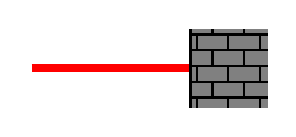
\begin{tikzpicture}
  \wall
  % The "line"
  \draw [red,line width=1mm] (-1,0) -- (1,0);
\end{tikzpicture}
\end{codeexample}

Now we wish to add a blue open arrow tip the red line like, say,
|Stealth[length=1cm,open,blue]|:
%
\begin{codeexample}[setup code,hidden]
\usetikzlibrary{patterns}
\def\wall{ \fill     [fill=black!50]  (1,-.5) rectangle (2,.5);
           \pattern  [pattern=bricks] (1,-.5) rectangle (2,.5);
           \draw     [line width=1pt]  (1cm+.5pt,-.5) -- ++(0,1); }
\end{codeexample}
\begin{codeexample}[preamble={\usetikzlibrary{arrows.meta}}]
\begin{tikzpicture}
  \wall
  \draw [red,line width=1mm,-{Stealth[length=1cm,open,blue]}]
        (-1,0) -- (1,0);
\end{tikzpicture}
\end{codeexample}

There are several noteworthy things about the blue arrow tip:
%
\begin{enumerate}
    \item Notice that the red line no longer goes all the way to the wall.
        Indeed, the red line ends more or less exactly where it meets the
        blue line, leaving the arrow tip empty. Now, recall that the red line
        was supposed to be the path |(-2,0)--(1,0)|; however, this path has
        obviously become much shorter (by 6.25mm to be precise). This effect
        is called \emph{path shortening} in \tikzname.
    \item The very tip of the arrow just ``touches'' the wall, even we zoom
        out a lot. This point, where the original path ended and where the
        arrow tip should now lie, is called the \emph{tip end} in \tikzname.
    \item Finally, the point where the red line touches the blue line is the
        point where the original path ``visually ends''. Notice that this is
        not the same as the point that lies at a distance of the arrow's
        |length| from the wall -- rather it lies at a distance of |length|
        minus the |inset|. Let us call this point the \emph{visual
    end} of the arrow.
\end{enumerate}

As pointed out earlier, for straight lines, shortening the path and rotating
and shifting the arrow tip so that it ends precisely at the tip end and the
visual end lies on a line from the tip end to the start of the line is
relatively easy.

For curved lines, things are much more difficult and \tikzname\ copes with the
difficulties in different ways, depending on which options you add to arrows.
Here is now a curved red line to which we wish to add our arrow tip (the
original straight red line is shown in light red):
%
\begin{codeexample}[]
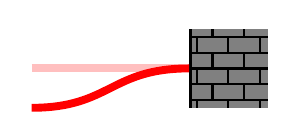
\begin{tikzpicture}
  \wall
  \draw [red!25,line width=1mm] (-1,0) -- (1,0);
  \draw [red,line width=1mm] (-1,-.5) .. controls (0,-.5) and (0,0) .. (1,0);
\end{tikzpicture}
\end{codeexample}

The first way of dealing with curved lines is dubbed the ``quick and dirty''
way (although the option for selecting this option is politely just called
``|quick|'' \dots):

\begin{key}{/pgf/arrow keys/quick}
    Recall that curves in \tikzname\ are actually Bézier curves, which means
    that they start and end at certain points and we specify two vectors, one
    for the start and one for the end, that provide tangents to the curve at
    these points. In particular, for the end of the curve, there is a point
    called the \emph{second support point} of the curve such that a tangent to
    the curve at the end goes through this point. In our above example, the
    second support point is at the middle of the light red line and, indeed, a
    tangent to the red line at the point touching the wall is perfectly
    horizontal.

    In order to add our arrow tip to the curved path, our first objective is to
    ``shorten'' the path by 6.25mm. Unfortunately, this is now much more
    difficult than for a straight path. When the |quick| option is added to an
    arrow tip (it is also the default if no special libraries are loaded), we
    cheat somewhat: Instead of really moving along 6.25mm along the path, we
    simply shift the end of the curve by 6.25mm \emph{along the tangent} (which
    is easy to compute). We also have to shift the second support point by the
    same amount to ensure that the line still has the same tangent at the end.
    This will result in the following:
    %
\begin{codeexample}[preamble={\usetikzlibrary{arrows.meta}}]
\begin{tikzpicture}
  \wall
  \draw [red!25,line width=1mm] (-1,0) -- (1,0);
  \draw [red,line width=1mm,-{Stealth[length=1cm,open,blue,quick]}]
        (-1,-.5) .. controls (0,-.5) and (0,0) .. (1,0);
\end{tikzpicture}
\end{codeexample}

    They main problem with the above picture is that the red line is no longer
    equal to the original red line (notice much sharper curvature near its
    end). In our example this is not such a bad thing, but it certainly ``not a
    nice thing'' that adding arrow tips to a curve changes the overall shape of
    the curves. This is especially bothersome if there are several similar
    curves that have different arrow heads. In this case, the similar curves
    now suddenly look different.

    Another big problem with the above approach is that it works only well if
    there is only a single arrow tip. When there are multiple ones, simply
    shifting them along the tangent as the |quick| option does produces
    less-than-satisfactory results:
    %
\begin{codeexample}[]
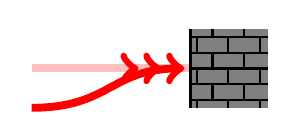
\begin{tikzpicture}
  \wall
  \draw [red!25,line width=1mm] (-1,0) -- (1,0);
  \draw [red,line width=1mm,-{[quick,sep]>>>}]
        (-1,-.5) .. controls (0,-.5) and (0,0) .. (1,0);
\end{tikzpicture}
\end{codeexample}
    %
    Note that the third arrow tip does not really lie on the curve any more.
\end{key}

Because of the shortcomings of the |quick| key, more powerful mechanisms for
shortening lines and rotating arrows tips have been implemented. To use them,
you need to load the following library:

\begin{tikzlibrary}{bending}
    Load this library to use the |flex|, |flex'|, or |bending| arrow keys. When
    this library is loaded, |flex| becomes the default mode that is used with
    all paths, unless |quick| is explicitly selected for the arrow tip.
\end{tikzlibrary}

\begin{key}{/pgf/arrow keys/flex=\opt{\meta{factor}} (default 1)}
    When the |bending| library is loaded, this key is applied to all arrow tips
    by default. It has the following effect:
    %
    \begin{enumerate}
        \item Instead of simply shifting the visual end of the arrow along
            the tangent of the curve's end, we really move it along the curve
            by the necessary distance. This operation is more expensive than
            the |quick| operation -- but not \emph{that} expensive, only
            expensive enough so that it is not selected by default for all
            arrow tips. Indeed, some compromises are made in the
            implementation where accuracy was traded for speed, so the
            distance by which the line end is shifted is not necessarily
            \emph{exactly} 6.25mm; only something reasonably close.
        \item The supports of the line are updated accordingly so that the
            shortened line will still follow \emph{exactly} the original
            line. This means that the curve deformation effect caused by the
            |quick| command does not happen here.
        \item Next, the arrow tip is rotated and shifted as follows: First,
            we shift it so that its tip is exactly at the tip end, where the
            original line ended. Then, the arrow is rotated so the \emph{the
            visual end lies on the line}:
            %
\begin{codeexample}[preamble={\usetikzlibrary{arrows.meta,bending}}]
\begin{tikzpicture}
  \wall
  \draw [red!25,line width=1mm] (-1,0) -- (1,0);
  \draw [red,line width=1mm,-{Stealth[length=1cm,open,blue,flex]}]
        (-1,-.5) .. controls (0,-.5) and (0,0) .. (1,0);
\end{tikzpicture}
\end{codeexample}
    \end{enumerate}

    As can be seen in the example, the |flex| option gives a result that is
    visually pleasing and does not deform the path.

    There is, however, one possible problem with the |flex| option: The arrow
    tip no longer points along the tangent of the end of the path. This may or
    may not be a problem, put especially for larger arrow tips readers will use
    the orientation of the arrow head to gauge the direction of the tangent of
    the line. If this tangent is important (for example, if it should be
    horizontal), then it may be necessary to enforce that the arrow tip
    ``really points in the direction of the tangent''.

    To achieve this, the |flex| option takes an optional \meta{factor}
    parameter, which defaults to |1|. This factor specifies how much the arrow
    tip should be rotated: If set to |0|, the arrow points exactly along a
    tangent to curve at its tip. If set to |1|, the arrow point exactly along a
    line from the visual end point on the curve to the tip. For values in the
    middle, we interpolate the rotation between these two extremes; so
    |flex=.5| will rotate the arrow's visual end ``halfway away from the
    tangent towards the actual position on the line''.
    %
\begin{codeexample}[preamble={\usetikzlibrary{arrows.meta,bending}}]
\begin{tikzpicture}
  \wall
  \draw [red!25,line width=1mm] (-1,0) -- (1,0);
  \draw [red,line width=1mm,-{Stealth[length=1cm,open,blue,flex=0]}]
        (-1,-.5) .. controls (0,-.5) and (0,0) .. (1,0);
\end{tikzpicture}
\end{codeexample}
\begin{codeexample}[preamble={\usetikzlibrary{arrows.meta,bending}}]
\begin{tikzpicture}
  \wall
  \draw [red!25,line width=1mm] (-1,0) -- (1,0);
  \draw [red,line width=1mm,-{Stealth[length=1cm,open,blue,flex=.5]}]
        (-1,-.5) .. controls (0,-.5) and (0,0) .. (1,0);
\end{tikzpicture}
\end{codeexample}
    %
    Note how in the above examples the red line is visible inside the open
    arrow tip. Open arrow tips do not go well with a flex value other than~|1|.
    Here is a more realistic use of the |flex=0| key:
    %
\begin{codeexample}[preamble={\usetikzlibrary{arrows.meta,bending}}]
\begin{tikzpicture}
  \wall
  \draw [red!25,line width=1mm] (-1,0) -- (1,0);
  \draw [red,line width=1mm,-{Stealth[length=1cm,flex=0]}]
        (-1,-.5) .. controls (0,-.5) and (0,0) .. (1,0);
\end{tikzpicture}
\end{codeexample}
    %
    If there are several arrow tips on a path, the |flex| option positions them
    independently, so that each of them lies optimally on the path:
    %
\begin{codeexample}[preamble={\usetikzlibrary{bending}}]
\begin{tikzpicture}
  \wall
  \draw [red!25,line width=1mm] (-1,0) -- (1,0);
  \draw [red,line width=1mm,-{[flex,sep]>>>}]
        (-1,-.5) .. controls (0,-.5) and (0,0) .. (1,0);
\end{tikzpicture}
\end{codeexample}
    %
\end{key}

\begin{key}{/pgf/arrow keys/flex'=\opt{\meta{factor}} (default 1)}
    The |flex'| key is almost identical to the |flex| key. The only difference
    is that a factor of |1| corresponds to rotating the arrow tip so that the
    instead of the visual end, the ``ultimate back end'' of the arrow tip lies
    on the red path. In the example instead of having the arrow tip at a
    distance of |6.25mm| from the tip lie on the path, we have the point at a
    distance of |1cm| from the tip lie on the path:
    %
\begin{codeexample}[preamble={\usetikzlibrary{arrows.meta,bending}}]
\begin{tikzpicture}
  \wall
  \draw [red!25,line width=1mm] (-1,0) -- (1,0);
  \draw [red,line width=1mm,-{Stealth[length=1cm,open,blue,flex']}]
        (-1,-.5) .. controls (0,-.5) and (0,0) .. (1,0);
\end{tikzpicture}
\end{codeexample}
    %
    Otherwise, the factor works as for |flex| and, indeed |flex=0| and
    |flex'=0| have the same effect.

    The main use of this option is not so much with an arrow tip like |Stealth|
    but rather with tips like the standard |>| in the context of a strongly
    curved line:
    %
\begin{codeexample}[preamble={\usetikzlibrary{arrows.meta,bending}}]
\begin{tikzpicture}
  \wall
  \draw [red!25,line width=1mm] (-1,0) -- (1,0);
  \draw [red,line width=1mm,-{Computer Modern Rightarrow[flex]}]
        (0,-.5) .. controls (1,-.5) and (0.5,0) .. (1,0);
\end{tikzpicture}
\end{codeexample}
    %
    In the example, the |flex| option does not really flex the arrow since for
    a tip like the Computer Modern arrow, the visual end is the same as the
    arrow tip -- after all, the red line does, indeed, end almost exactly where
    it used to end.

    Nevertheless, you may feel that the arrow tip looks ``wrong'' in the sense
    that it should be rotated. This is exactly what the |flex'| option does
    since it allows us to align the ``back end'' of the tip with the red line:
    %
\begin{codeexample}[preamble={\usetikzlibrary{arrows.meta,bending}}]
\begin{tikzpicture}
  \wall
  \draw [red!25,line width=1mm] (-1,0) -- (1,0);
  \draw [red,line width=1mm,-{Computer Modern Rightarrow[flex'=.75]}]
        (0,-.5) .. controls (1,-.5) and (0.5,0) .. (1,0);
\end{tikzpicture}
\end{codeexample}
    %
    In the example, I used |flex'=.75| so as not to overpronounce the effect.
    Usually, you will have to fiddle with it sometime to get the ``perfectly
    aligned arrow tip'', but a value of |.75| is usually a good start.
\end{key}

\begin{key}{/pgf/arrow keys/bend}
    \emph{Bending} an arrow tip is a radical solution to the problem of
    positioning arrow tips on a curved line: The arrow tip is no longer
    ``rigid'' but the drawing itself will now bend along the curve. This has
    the advantage that all the problems of flexing with wrong tangents and
    overflexing disappear. The downsides are longer computation times (bending
    an arrow is \emph{much} more expensive that flexing it, let alone than
    quick mode) and also the fact that excessive bending can lead to ugly arrow
    tips. On the other hand, for most arrow tips their bend version are
    visually quite pleasing and create a sophisticated look:
    %
\begin{codeexample}[preamble={\usetikzlibrary{arrows.meta,bending}}]
\begin{tikzpicture}
  \wall
  \draw [red!25,line width=1mm] (-1,0) -- (1,0);
  \draw [red,line width=1mm,-{Stealth[length=20pt,bend]}]
        (-1,-.5) .. controls (0,-.5) and (0,0) .. (1,0);
\end{tikzpicture}
\end{codeexample}
\begin{codeexample}[preamble={\usetikzlibrary{bending}}]
\begin{tikzpicture}
  \wall
  \draw [red!25,line width=1mm] (-1,0) -- (1,0);
  \draw [red,line width=1mm,-{[bend,sep]>>>}]
        (-1,-.5) .. controls (0,-.5) and (0,0) .. (1,0);
\end{tikzpicture}
\end{codeexample}
\begin{codeexample}[preamble={\usetikzlibrary{arrows.meta,bending}}]
\begin{tikzpicture}
  \wall
  \draw [red!25,line width=1mm] (-1,0) -- (1,0);
  \draw [red,line width=1mm,-{Stealth[bend,round,length=20pt]}]
        (0,-.5) .. controls (1,-.5) and (0.25,0) .. (1,0);
\end{tikzpicture}
\end{codeexample}
    %
\end{key}
% TODOsp: codeexamples: `bending` library is needed up to here
% TODOsp: codeexamples: `\def\wall` + `patterns` library are needed up to here
% TODOsp: codeexamples: `arrows.meta` library needed up to here


\subsection{Arrow Tip Specifications}
\label{section-arrow-spec}

\subsubsection{Syntax}

When you select the arrow tips for the start and the end of a path, you can
specify a whole sequence of arrow tips, each having its own local options. At
the beginning of this section, it was pointed out that the syntax for selecting
the start and end arrow tips is the following:
%
\begin{quote}
    \meta{start specification}|-|\meta{end specification}
\end{quote}

We now have a closer look at what these specifications may look like. The
general syntax of the \meta{start specification} is as follows:
%
\begin{quote}
    \opt{|[|\meta{options for all tips}|]|} \meta{first arrow tip spec}
    \meta{second arrow tip spec} \meta{third arrow tip spec} \dots
\end{quote}
%
As can be seen, an arrow tip specification may start with some options in
brackets. If this is the case, the \meta{options for all tips} will, indeed, be
applied to all arrow tips that follow. (We will see, in a moment, that there
are even more places where options may be specified and a list of the ordering
in which the options are applied will be given later.)

The main part of a specification is taken up by a sequence of individual arrow
tip specifications. Such a specification can be of three kinds:
%
\begin{enumerate}
    \item It can be of the form \meta{arrow tip kind
        name}|[|\meta{options}|]|.
    \item It can be of the form \meta{shorthand}|[|\meta{options}|]|.
    \item It can be of the form \meta{single char
        shorthand}\opt{|[|\meta{options}|]|}. Note that only for this form
        the brackets are optional.
\end{enumerate}

The easiest kind is the first one: This adds an arrow tip of the kind
\meta{arrow tip kind name} to the sequence of arrow tips with the
\meta{options} applied to it at the start (for the \meta{start specification})
or at the end (for the \meta{end specification}). Note that for the \meta{start
specification} the first arrow tip specified in this way will be at the very
start of the curve, while for the \meta{end specification} the ordering is
reversed: The last arrow tip specified will be at the very end of the curve.
This implies that a specification like
%
\begin{quote}
    |Stealth[] Latex[] - Latex[] Stealth[]|
\end{quote}
%
will give perfectly symmetric arrow tips on a line (as one would expect).

It is important that even if there are no \meta{options} for an arrow tip, the
square brackets still need to be written to indicate the end of the arrow tip's
name. Indeed, the opening brackets are used to divide the arrow tip
specification into names.

Instead of a \meta{arrow tip kind name}, you may also provide the name of a
so-called \emph{shorthand}. Shorthands look like normal arrow tip kind names
and, indeed, you will often be using shorthands without noticing that you do.
The idea is that instead of, say, |Computer Modern Rightarrow| you might wish
to just write |Rightarrow| or perhaps just |To| or even just |>|. For this, you
can create a shorthand that tells \tikzname\ that whenever this shorthand is
used, another arrow tip kind is meant. (Actually, shorthands are somewhat more
powerful, we have a detailed look at them in
Section~\ref{section-arrow-tip-macro}.) For shorthands, the same rules apply as
for normal arrow tip kinds: You \emph{need} to provide brackets so that
\tikzname\ can find the end of the name inside a longer specification.

The third kind of arrow tip specifications consist of just a single letter like
|>| or |)| or |*| or even |o| or |x| (but you may not use |[|, |]|, or |-|
since they will confuse the parser). These single letter arrow specifications
will invariably be shorthands that select some ``real'' arrow tip instead. An
important feature of single letter arrow tips is that they do \emph{not} need
to be followed by options (but they may).

Now, since we can use any letter for single letter shorthands, how can
\tikzname\ tell whether by |foo[]| we mean an arrow tip kind |foo| without any
options or whether we mean an arrow tip called |f|, followed by two arrow tips
called |o|? Or perhaps an arrow tip called |f| followed by an arrow tip called
|oo|? To solve this problem, the following rule is used to determine which of
the three possible specifications listed above applies: First, we check whether
everything from the current position up to the next opening bracket (or up to
the end) is the name of an arrow tip or of a shorthand. In our case, |foo|
would first be tested under this rule. Only if |foo| is neither the name of an
arrow tip kind nor of a shorthand does \tikzname\ consider the first letter of
the specification, |f| in our case. If this is not the name of a shorthand, an
error is raised. Otherwise the arrow tip corresponding to |f| is added to the
list of arrow tips and the process restarts with the rest. Thus, we would next
text whether |oo| is the name of an arrow tip or shorthand and, if not, whether
|o| is such a name.

All of the above rules mean that you can rather easily specify arrow tip
sequences if they either mostly consist of single letter names or of longer
names. Here are some examples:
%
\begin{itemize}
    \item |->>>| is interpreted as three times the |>| shorthand since |>>>| is
        not the name of any arrow tip kind (and neither is |>>|).
    \item |->[]>>| has the same effect as the above.
    \item |-[]>>>| also has the same effect.
    \item |->[]>[]>[]| so does this.
    \item |->Stealth| yields an arrow tip |>| followed by a |Stealth| arrow
        at the end.
    \item |-Stealth>| is illegal since there is no arrow tip |Stealth>| and
        since |S| is also not the name of any arrow tip.
    \item |-Stealth[] >| is legal and does what was presumably meant in the
        previous item.
    \item |< Stealth-| is legal and is the counterpart to |-Stealth[] >|.
    \item |-Stealth[length=5pt] Stealth[length=6pt]| selects two stealth
        arrow tips, but at slightly different sizes for the end of lines.
\end{itemize}

An interesting question concerns how flexing and bending interact with multiple
arrow tips: After all, flexing and quick mode use different ways of shortening
the path so we cannot really mix them. The following rule is used: We check,
independently for the start and the end specifications, whether at least one
arrow tip in them uses one of the options |flex|, |flex'|, or |bend|. If so,
all |quick| settings in the other arrow tips are ignored and treated as if
|flex| had been selected for them, too.


\subsubsection{Specifying Paddings}

When you provide several arrow tips in a row, all of them are added to the
start or end of the line:
%
\begin{codeexample}[]
\tikz \draw [<<<->>>>] (0,0) -- (2,0);
\end{codeexample}
%
The question now is what will be the distance between them? For this, the
following arrow key is important:

\begin{key}{/pgf/arrow keys/sep=\meta{dimension}| |\opt{\meta{line
    width factor}}| |\opt{\meta{outer factor}} (default 0.88pt .3 1)%
}
    When a sequence of arrow tips is specified in an arrow tip specification
    for the end of the line, the arrow tips are normally arranged in such a way
    that the tip of each arrow ends exactly at the ``back end'' of the next
    arrow tip (for start specifications, the ordering is inverted, of course).
    Now, when the |sep| option is set, instead of exactly touching the back end
    of the next arrow, the specified \meta{dimension} is added as additional
    space (the distance may also be negative, resulting in an overlap of the
    arrow tips). The optional factors have the same meaning as for the |length|
    key, see that key for details.

    Let us now have a look at some examples. First, we use two arrow tips with
    different separations between them:
    %
\begin{codeexample}[preamble={\usetikzlibrary{arrows.meta}}]
\tikz {
  \draw [-{>[sep=1pt]>[sep= 2pt]>}] (0,1.0) -- (1,1.0);
  \draw [-{>[sep=1pt]>[sep=-2pt]>}] (0,0.5) -- (1,0.5);
  \draw [-{>         >[sep]     >}] (0,0.0) -- (1,0.0);
}
\end{codeexample}

    You can also specify a |sep| for the last arrow tip in the sequence (for
    end specifications, otherwise for the first arrow tip). In this case, this
    first arrow tip will not exactly ``touch'' the point where the path ends,
    but will rather leave the specified amount of space. This is usually quite
    desirable.
    %
\begin{codeexample}[preamble={\usetikzlibrary{arrows.meta,positioning}}]
\tikz {
  \node [draw] (A) {A};
  \node [draw] (B) [right=of A] {B};

  \draw [-{>>[sep=2pt]}] (A) to [bend left=45] (B);
  \draw [- >>          ] (A) to [bend right=45] (B);
}
\end{codeexample}
    %
    Indeed, adding a |sep| to an arrow tip is \emph{very} desirable, so you
    will usually write something like |>={To[sep]}| somewhere near the start of
    your files.

    One arrow tip kind can be quite useful in this context: The arrow tip kind
    |_|. It draws nothing and has zero length, \emph{but} it has |sep| set as a
    default option. Since it is a single letter shorthand, you can write short
    and clean ``code'' in this way:
    %
\begin{codeexample}[]
\tikz \draw [->_>] (0,0) -- (1,0);
\end{codeexample}
\begin{codeexample}[]
\tikz \draw [->__>] (0,0) -- (1,0);
\end{codeexample}
    %
    However, using the |sep| option will be faster than using the |_| arrow tip
    and it also allows you to specify the desired length directly.
\end{key}


\subsubsection{Specifying the Line End}

In the previous examples of sequences of arrow tips, the line of the path
always ended at the last of the arrow tips (for end specifications) or at the
first of the arrow tips (for start specifications). Often, this is what you may
want, but not always. Fortunately, it is quite easy to specify the desired end
of the line: The special single char shorthand |.| is reserved to indicate that
last arrow that is still part of the line; in other words, the line will stop
at the last arrow before |.| is encountered (for end specifications) are at the
first arrow following |.| (for start specifications).
%
\begin{codeexample}[]
\tikz [very thick] \draw [<<<->>>] (0,0) -- (2,0);
\end{codeexample}
\begin{codeexample}[]
\tikz [very thick] \draw [<.<<->.>>] (0,0) -- (2,0);
\end{codeexample}
\begin{codeexample}[]
\tikz [very thick] \draw [<<.<-.>>>] (0,0) -- (2,0);
\end{codeexample}
\begin{codeexample}[]
\tikz [very thick] \draw [<<.<->.>>] (0,0) to [bend left] (2,0);
\end{codeexample}

It is permissible that there are several dots in a specification, in this case
the first one ``wins'' (for end specifications, otherwise the last one).

Note that |.| is parsed as any other shorthand. In particular, if you wish to
add a dot after a normal arrow tip kind name, you need to add brackets:
%
\begin{codeexample}[preamble={\usetikzlibrary{arrows.meta}}]
\tikz [very thick] \draw [-{Stealth[] . Stealth[] Stealth[]}] (0,0) -- (2,0);
\end{codeexample}
%
Adding options to |.| is permissible, but they have no effect. In particular,
|sep| has no effect since a dot is not an arrow.


\subsubsection{Defining Shorthands}
\label{section-arrow-tip-macro}

It is often desirable to create ``shorthands'' for the names of arrow tips that
you are going to use very often. Indeed, in most documents you will only need a
single arrow tip kind and it would be useful that you could refer to it just as
|>| in your arrow tip specifications. As another example, you might constantly
wish to switch between a filled and a non-filled circle as arrow tips and would
like to use |*| and |o| are shorthands for these case. Finally, you might just
like to shorten a long name like |Computer Modern Rightarrow| down to just, say
|To| or something similar.

All of these case can be addressed by defining appropriate shorthands. This is
done using the following handler:

\begin{handler}{{.tip}{=\meta{end specification}}}
    Defined the \meta{key} as a name that can be used inside arrow tip
    specifications. If the \meta{key} has a path before it, this path is
    ignored (so there is only one ``namespace'' for arrow tips). Whenever it is
    used, it will be replaced by the \meta{end specification}. Note that you
    must \emph{always} provide (only) an end specification; when the \meta{key}
    is used inside a start specification, the ordering and the meaning of the
    keys inside the \meta{end specification} are translated automatically.
    \todosp{remaining instance of bug \#473}
    %
\begin{codeexample}[preamble={\usetikzlibrary{arrows.meta}}]
\tikz [foo /.tip = {Stealth[sep]. >>}]
  \draw [-foo] (0,0) -- (2,0);
\end{codeexample}
\begin{codeexample}[preamble={\usetikzlibrary{arrows.meta}}]
\tikz [foo /.tip = {Stealth[sep] Latex[sep]},
       bar /.tip = {Stealth[length=10pt,open]}]
  \draw [-{foo[red] . bar}] (0,0) -- (2,0);
\end{codeexample}

    In the last of the examples, we used |foo[red]| to make the arrows red. Any
    options given to a shorthand upon use will be passed on to the actual
    arrows tip for which the shorthand stands. Thus, we could also have written
    |Stealth[sep,red]| |Latex[sep,red]| instead of |foo[red]|. In other words,
    the ``replacement'' of a shorthand by its ``meaning'' is a semantic
    replacement rather than a syntactic replacement. In particular, the
    \meta{end specification} will be parsed immediately when the shorthand is
    being defined. However, this applies only to the options inside the
    specification, whose values are evaluated immediately. In contrast, which
    actual arrow tip kind is meant by a given shorthand used inside the
    \meta{end specification} is resolved only up each use of the shorthand.
    This means that when you write
    %
    \begin{quote}
        |dup /.tip = >>|
    \end{quote}
    %
    and then later write
    %
    \begin{quote}
        |> /.tip = whatever|
    \end{quote}
    %
    then |dup| will have the effect as if you had written
    |whatever[]whatever[]|. You will find that this behavior is what one would
    expect.

    There is one problem we have not yet addressed: The asymmetry of single
    letter arrow tips like |>| or |)|. When someone writes
    %
\begin{codeexample}[]
\tikz \draw [<->] (0,0) -- (1,0);
\end{codeexample}
    %
    we rightfully expect one arrow tip pointing left at the left end and an
    arrow tip pointing right at the right end. However, compare
    %
\begin{codeexample}[]
\tikz \draw [>->] (0,0) -- (1,0);
\end{codeexample}
\begin{codeexample}[preamble={\usetikzlibrary{arrows.meta}}]
\tikz \draw [Stealth-Stealth] (0,0) -- (1,0);
\end{codeexample}
    %
    In both cases, we have \emph{identical} text in the start and end
    specifications, but in the first case we rightfully expect the left arrow
    to be flipped.

    The solution to this problem is that it is possible to define two names for
    the same arrow tip, namely one that is used inside start specifications and
    one for end specifications. Now, we can decree that the ``name of |>|''
    inside start specifications is simply |<| and the above problems disappear.

    To specify different names for a shorthand in start and end specifications,
    use the following syntax: Instead of \meta{key}, you use \meta{name in
    start specifications}|-|\meta{name in end specifications}. Thus, to set the
    |>| key correctly, you actually need to write
    %
\begin{codeexample}[preamble={\usetikzlibrary{arrows.meta}}]
\tikz [<-> /.tip = Stealth] \draw [<->>] (0,0) -- (1,0);
\end{codeexample}
\begin{codeexample}[preamble={\usetikzlibrary{arrows.meta}}]
\tikz [<-> /.tip = Latex] \draw [>-<] (0,0) -- (1,0);
\end{codeexample}

    Note that the above also works even though we have not set |<| as an arrow
    tip name for end specifications! The reason this works is that the
    \tikzname\ (more precisely, \pgfname) actually uses the following
    definition internally:
    %
    \begin{quote}
        |>-< /.tip = >[reversed]|
    \end{quote}
    %
    Translation: ``When |<| is used in an end specification, please replace it
    by |>|, but reversed. Also, when |>| is used in a start specification, we
    also mean this inverted |>|.''

    By default, |>| is a shorthand for |To| and |To| is a shorthand for |to|
    (an arrow from the old libraries) when |arrows.meta| is not loaded library.
    When |arrows.meta| is loaded, |To| is redefined to mean the same as
    |Computer Modern Rightarrow|.
\end{handler}

\begin{key}{/tikz/>=\meta{end arrow specification}}
    This is a short way of saying |<->/.tip=|\meta{end arrow specification}.
    %
\begin{codeexample}[preamble={\usetikzlibrary{arrows.meta}}]
\begin{tikzpicture}[scale=2,ultra thick]
  \begin{scope}[>=Latex]
    \draw[>->]    (0pt,3ex) -- (1cm,3ex);
    \draw[|<->>|] (0pt,2ex) -- (1cm,2ex);
  \end{scope}
  \begin{scope}[>=Stealth]
    \draw[>->]    (0pt,1ex) -- (1cm,1ex);
    \draw[|<<.<->|] (0pt,0ex) -- (1cm,0ex);
  \end{scope}
\end{tikzpicture}
\end{codeexample}
    %
\end{key}

\begin{key}{/tikz/shorten <=\meta{length}}
    Shorten the path by \meta{length} in the direction of the starting point.
\end{key}

\begin{key}{/tikz/shorten >=\meta{length}}
    Shorten the path by \meta{length} in the direction of the end point.
\end{key}


\subsubsection{Scoping of Arrow Keys}
\label{section-arrow-scopes}

There are numerous places where you can specify keys for an arrow tip. There
is, however, one final place that we have not yet mentioned:

\begin{key}{/tikz/arrows=|[|\meta{arrow keys}|]|}
    The |arrows| key, which is normally used to set the arrow tips for the
    current scope, can also be used to set some arrow keys for the current
    scope. When the argument to |arrows| starts with an opening bracket and
    only otherwise contains one further closing bracket at the very end, this
    semantic of the |arrow| key is assumed.

    The \meta{arrow keys} will be set for the rest of current scope. This is
    useful for generally setting some design parameters or for generally
    switching on, say, bending as in:
    %
\begin{codeexample}[code only]
\tikz [arrows={[bend]}] ... % Bend all arrows
\end{codeexample}
    %
\end{key}

We can now summarize which arrow keys are applied in what order when an arrow
tip is used:
%
\begin{enumerate}
    \item First, the so-called \emph{defaults} are applied, which are values
        for the different parameters of a key. They are fixed in the
        definition of the key and cannot be changed. Since they are executed
        first, they are only the ultimate fallback.
    \item The \meta{keys} from the use of |arrows=[|\meta{keys}|]| in all
        enclosing scopes.
    \item Recursively, the \meta{keys} provided with the arrow tip inside
        shorthands.
    \item The keys provided at the beginning of an arrow tip specification in
        brackets.
    \item The keys provided directly next to the arrow tip inside the
        specification.
\end{enumerate}


\subsection{Reference: Arrow Tips}
\label{section-arrows-meta}

\begin{pgflibrary}{arrows.meta}
    This library defines a large number of standard ``meta'' arrow tips.
    ``Meta'' means that you can configure these arrow tips in many different
    ways like changing their size or their line caps and joins and many other
    details.

    The only reason this library is not loaded by default is for compatibility
    with older versions of \tikzname. You can, however, safely load and use
    this library alongside the older libraries |arrows| and |arrows.spaced|.
\end{pgflibrary}

The different arrow tip kinds defined in the |arrows.meta| library can be
classified in different groups:
%
\begin{itemize}
    \item \emph{Barbed} arrow tips consist mainly of lines that ``point
        backward'' from the tip of the arrow and which are not filled. For
        them, filling has no effect. A typical example is \tikz [baseline]
        \draw (0,.5ex) -- (1.5em,.5ex) [-Straight Barb];. Here is the list of
        defined arrow tips:
        %
        \begin{arrowexamples}
            \arrowexample Arc Barb[]
            \arrowexample Bar[]
            \arrowexample Bracket[]
            \arrowexample Hooks[]
            \arrowexample Parenthesis[]
            \arrowexample Straight Barb[]
            \arrowexample Tee Barb[]
        \end{arrowexamples}

        All of these arrow tips can be configured and resized in many different
        ways as described in the following. Above, they are shown at their
        ``natural'' sizes, which are chosen in such a way that for a line width
        of 0.4pt their width matches the height of a letter ``x'' in Computer
        Modern at 11pt (with some ``overshooting'' to create visual
        consistency).
    \item \emph{Mathematical} arrow tips are actually a subclass of the
        barbed arrow tips, but we list them separately. They contain arrow
        tips that look exactly like the tips of arrows used in mathematical
        fonts such as the |\to|-symbol $\to$ from standard \TeX.
        %
        \begin{arrowexamples}
            \arrowexample Classical TikZ Rightarrow[]
            \arrowexample Computer Modern Rightarrow[]
            \arrowexampledouble Implies[]
            \arrowexample To[]
        \end{arrowexamples}
        %
        The |To| arrow tip is a shorthand for |Computer Modern Rightarrow| when
        |arrows.meta| is loaded.
    \item \emph{Geometric} arrow tips consist of a filled shape like a kite
        or a circle or a ``stealth-fighter-like'' shape. A typical example is
        \tikz [baseline] \draw (0,.5ex) -- (1.5em,.5ex) [-Stealth];. These
        arrow tips can also be used in an ``open'' variant as in \tikz
        [baseline] \draw (0,.5ex) -- (1.5em,.5ex) [-{Stealth[open]}];.
        %
        \begin{arrowexamples}
            \arrowexample Circle[]
            \arrowexample Diamond[]
            \arrowexample Ellipse[]
            \arrowexample Kite[]
            \arrowexample Latex[]
            \arrowexample Latex[round]
            \arrowexample Rectangle[]
            \arrowexample Square[]
            \arrowexample Stealth[]
            \arrowexample Stealth[round]
            \arrowexample Triangle[]
            \arrowexample Turned Square[]
        \end{arrowexamples}

        Here are the ``open'' variants:
        %
        \begin{arrowexamples}
            \arrowexample Circle[open]
            \arrowexample Diamond[open]
            \arrowexample Ellipse[open]
            \arrowexample Kite[open]
            \arrowexample Latex[open]
            \arrowexample Latex[round,open]
            \arrowexample Rectangle[open]
            \arrowexample Square[open]
            \arrowexample Stealth[open]
            \arrowexample Stealth[round,open]
            \arrowexample Triangle[open]
            \arrowexample Turned Square[open]
        \end{arrowexamples}

        Note that ``open'' arrow tips are not the same as ``filled with
        white'', which is also available (just say |fill=white|). The
        difference is that the background will ``shine through'' an open
        arrow, while a filled arrow always obscures the background:
        %
\begin{codeexample}[preamble={\usetikzlibrary{arrows.meta}}]
\tikz {
  \shade [left color=white, right color=red!50] (0,0) rectangle (4,1);

  \draw [ultra thick,-{Triangle[open]}]       (0,2/3) -- ++ (3,0);
  \draw [ultra thick,-{Triangle[fill=white]}] (0,1/3) -- ++ (3,0);
}
\end{codeexample}

    \item \emph{Cap} arrow tips are used to add a ``cap'' to the end of a
        line. The graphic languages underlying \tikzname\ (\textsc{pdf},
        \textsc{postscript} or \textsc{svg}) all support three basic types of
        line caps on a very low level: round, rectangular, and ``butt''.
        Using cap arrow tips, you can add new caps to lines and use different
        caps for the end and the start. An example is the line \tikz
        [baseline] \draw [line width=1ex, {Round Cap[reversed]}-{Triangle
        Cap[] . Fast Triangle[] Fast Triangle[]}] (0,0.5ex) -- (2em,0.5ex);.
        %
        \begin{arrowcapexamples}
            \arrowcapexample Butt Cap[]
            \arrowcapexample Fast Round[]
            \arrowcapexample Fast Triangle[]
            \arrowcapexample Round Cap[]
            \arrowcapexample Triangle Cap[]
        \end{arrowcapexamples}
    \item \emph{Special} arrow tips are used for some specific purpose and do
        not fit into the above categories.
        %
        \begin{arrowexamples}
            \arrowexample Rays[]
            \arrowexample Rays[n=8]
        \end{arrowexamples}
\end{itemize}


\subsubsection{Barbed Arrow Tips}

\begin{arrowtip}{Arc Barb}{
    This arrow tip attaches an arc to the end of the line whose angle is given
    by the |arc| option. The |length| and |width| parameters refer to the size
    of the arrow tip for |arc| set to 180 degrees, which is why in the example
    for |arc=210| the actual length is larger than the specified |length|. The
    line width is taken into account for the computation  of the length and
    width. Use the |round| option to add round caps to the end of the arcs.
}%
{length=1.5cm,arc=210}%
{length=1.5cm,width=3cm}

    \begin{arrowexamples}
        \arrowexample[]
        \arrowexampledup[sep]
        \arrowexampledupdot[sep]
        \arrowexample[arc=120]
        \arrowexample[arc=270]
        \arrowexample[length=2pt]
        \arrowexample[length=2pt,width=5pt]
        \arrowexample[line width=2pt]
        \arrowexample[reversed]
        \arrowexample[round]
        \arrowexample[slant=.3]
        \arrowexample[left]
        \arrowexample[right]
        \arrowexample[harpoon,reversed]
        \arrowexample[red]
    \end{arrowexamples}
    %
    The following options have no effect: |open|, |fill|.

    On |double| lines, the arrow tip will not look correct.
\end{arrowtip}

\begin{arrowtipsimple}{Bar}
    A simple bar. This is a simple instance of |Tee Barb| for length zero.
\end{arrowtipsimple}

\begin{arrowtip}{Bracket}{
    This is an instance of the |Tee Barb| \todosp{no space shown here} arrow tip that results in something
    resembling a bracket. Just like the |Parenthesis| arrow tip, a |Bracket| is
    not modelled from a text square bracket, but rather its size has been
    chosen so that it fits with the other arrow tips.
}%
{}%
{}

    \begin{arrowexamples}
        \arrowexample[]
        \arrowexampledup[sep]
        \arrowexampledupdot[sep]
        \arrowexample[reversed]
        \arrowexample[round]
        \arrowexample[slant=.3]
        \arrowexample[left]
        \arrowexample[right]
        \arrowexample[harpoon,reversed]
        \arrowexample[red]
    \end{arrowexamples}
    %
    The following options have no effect: |open|, |fill|.

    On |double| lines, the arrow tip will not look correct.
\end{arrowtip}

\begin{arrowtip}{Hooks}{
    This arrow tip attaches two ``hooks'' to the end of the line. The |length|
    and |width| parameters refer to the size of the arrow tip if both arcs are
    180 degrees; in the example the arc is 210 degrees and, thus, the arrow is
    actually longer that the |length| dictates. The line width is taken into
    account for the computation of the length and width. The |arc| option is
    used to specify the angle of the arcs. Use the |round| option to add round
    caps to the end of the arcs.
}%
{length=1cm,width=3.5cm,arc=210}%
{length=1cm,width=3.5cm}

    \begin{arrowexamples}
        \arrowexample[]
        \arrowexampledup[sep]
        \arrowexampledupdot[sep]
        \arrowexample[arc=120]
        \arrowexample[arc=270]
        \arrowexample[length=2pt]
        \arrowexample[length=2pt,width=5pt]
        \arrowexample[line width=2pt]
        \arrowexample[reversed]
        \arrowexample[round]
        \arrowexample[slant=.3]
        \arrowexample[left]
        \arrowexample[right]
        \arrowexample[harpoon,reversed]
        \arrowexample[red]
    \end{arrowexamples}
    %
    The following options have no effect: |open|, |fill|.

    On |double| lines, the arrow tip will not look correct.
\end{arrowtip}

\begin{arrowtip}{Parenthesis}{
    This arrow tip is an instantiation of the |Arc Barb| \todosp{no space shown here} so that it resembles a
    parenthesis. However, the idea is not to recreate a ``real'' parenthesis as
    it is used in text, but rather a ``bow'' at a size that harmonizes with the
    other arrow tips at their default sizes.
}%
{}%
{}

    \begin{arrowexamples}
        \arrowexample[]
        \arrowexampledup[sep]
        \arrowexampledupdot[sep]
        \arrowexample[reversed]
        \arrowexample[round]
        \arrowexample[slant=.3]
        \arrowexample[left]
        \arrowexample[right]
        \arrowexample[harpoon,reversed]
        \arrowexample[red]
    \end{arrowexamples}
    %
    The following options have no effect: |open|, |fill|.

    On |double| lines, the arrow tip will not look correct.
\end{arrowtip}

\begin{arrowtip}{Straight Barb}{
    This is the ``archetypal'' arrow head, consisting of just two straight
    lines. The |length| and |width| parameters refer to the horizontal and
    vertical distances between the points on the path making up the arrow tip.
    As can be seen, the line width of the arrow tip's path is not taken into
    account. The |angle| option is particularly useful to set the opening angle
    at the tip of the arrow head. The |round| option gives a ``softer'' or
    ``rounder'' version of the arrow tip.
}%
{length=2cm,width=3cm}%
{length=2cm/-4mm,width=3cm}

    \begin{arrowexamples}
        \arrowexample[]
%        \arrowexampledouble[]
        \arrowexampledup[]
        \arrowexampledupdot[]
        \arrowexample[length=5pt]
        \arrowexample[length=5pt,width=5pt]
        \arrowexample[line width=2pt]
        \arrowexample[reversed]
        \arrowexample[angle=60:2pt 3]
        \arrowexample[round]
        \arrowexample[slant=.3]
        \arrowexample[left]
        \arrowexample[right]
        \arrowexample[harpoon,reversed]
        \arrowexample[red]
    \end{arrowexamples}
    %
    The following options have no effect: |open|, |fill|.

    On |double| lines, the arrow tip will not look correct.
\end{arrowtip}

\begin{arrowtip}{Tee Barb}{
    This arrow tip attaches a little ``T'' on both sides of the tip. The arrow
    |inset| dictates the distance from the back end to the middle of the stem
    of the T. When the inset is equal to the length, the arrow tip is drawn as
    a single line, not as three lines (this is important for the ``round''
    version since, then, the corners get rounded).
}%
{length=1.5cm,width=3cm,inset=1cm}%
{length=1.5cm,width=3cm,inset=1cm}

    \begin{arrowexamples}
        \arrowexample[]
        \arrowexampledup[sep]
        \arrowexampledupdot[sep]
        \arrowexample[inset=0pt]
        \arrowexample[inset'=0pt 1]
        \arrowexample[line width=2pt]
        \arrowexample[round]
        \arrowexample[round,inset'=0pt 1]
        \arrowexample[slant=.3]
        \arrowexample[left]
        \arrowexample[right]
        \arrowexample[harpoon,reversed]
        \arrowexample[red]
    \end{arrowexamples}
    %
    The following options have no effect: |open|, |fill|.

    On |double| lines, the arrow tip will not look correct.
\end{arrowtip}


\subsubsection{Mathematical Barbed Arrow Tips}

\begin{arrowtip}{Classical TikZ Rightarrow}{
    This arrow tip is the ``old'' or ``classical'' arrow tip that used to be
    the standard in \tikzname\ in earlier versions. It was modelled on an old
    version of the tip of \texttt{\string\rightarrow} ($\rightarrow$) of the
    Computer Modern fonts. However, this ``old version'' was really old, Donald
    Knuth (the designer of both \TeX\ and of the Computer Modern fonts)
    replaced the arrow tip of the mathematical fonts in~1992.
}%
{length=1cm,width=2cm}%
{length=1cm,width=2cm}

    The main problem with this arrow tip is that it is ``too small'' at its
    natural size. I recommend using the new \texttt{Computer Modern Rightarrow}
    arrow tip instead, which matches the current $\to$. This new version is
    also the default used as |>| and as |To|, now.
    %
    \begin{arrowexamples}
        \arrowexample[]
        \arrowexampledup[sep]
        \arrowexampledupdot[sep]
        \arrowexample[length=3pt]
        \arrowexample[sharp]
        \arrowexample[slant=.3]
        \arrowexample[left]
        \arrowexample[right]
        \arrowexample[harpoon,reversed]
        \arrowexample[red]
    \end{arrowexamples}
    %
    The following options have no effect: |open|, |fill|.

    On |double| lines, the arrow tip will not look correct.
\end{arrowtip}

\begin{arrowtip}{Computer Modern Rightarrow}{
    For a line width of 0.4pt (the default), this arrow tip looks very much
    like \texttt{\string\rightarrow} ($\to$) of the Computer Modern math fonts.
    However, it is not a ``perfect'' match: the line caps and joins of the
    ``real'' $\to$ are rounded differently from this arrow tip; but it takes a
    keen eye to notice the difference. When the |arrows.meta| library is loaded,
    this arrow tip becomes the default of |To| and, thus, is used whenever |>|
    is used (unless, of course, you redefined |>|).
}%
{length=1cm,width=2cm}%
{length=1cm,width=2cm}

    \begin{arrowexamples}
        \arrowexample[]
        \arrowexampledup[sep]
        \arrowexampledupdot[sep]
        \arrowexample[length=3pt]
        \arrowexample[sharp]
        \arrowexample[slant=.3]
        \arrowexample[left]
        \arrowexample[right]
        \arrowexample[harpoon,reversed]
        \arrowexample[red]
    \end{arrowexamples}
    %
    The following options have no effect: |open|, |fill|.

    On |double| lines, the arrow tip will not look correct.
\end{arrowtip}

\begin{arrowtipsimple}{Implies}
    This arrow tip makes only sense in conjunction with the |double| option.
    The idea is that you attach it to a double line to get something that looks
    like \TeX's \texttt{\string\implies} arrow ($\implies$). A typical use of
    this arrow tip is
    %
\begin{codeexample}[preamble={\usetikzlibrary{arrows.meta,graphs}}]
\tikz \graph [clockwise=3, math nodes,
              edges = {double equal sign distance, -Implies}] {
  "\alpha", "\beta", "\gamma";
  "\alpha" -> "\beta" -> "\gamma" -> "\alpha"
};
\end{codeexample}
    %
    \begin{arrowexamples}
        \arrowexampledouble[]
        \arrowexampledouble[red]
    \end{arrowexamples}
\end{arrowtipsimple}

\begin{arrowtipsimple}{To}
    This is a shorthand for |Computer Modern Rightarrow| when the |arrows.meta|
    library is loaded. Otherwise, it is a shorthand for the classical
    \tikzname\ rightarrow.
\end{arrowtipsimple}


\subsubsection{Geometric Arrow Tips}

\begin{arrowtip}{Circle}{
    Although this tip is called ``circle'', you can also use it to draw
    ellipses if you set the length and width to different values. Neither
    |round| nor |reversed| has any effect on this arrow tip.
}%
{length=2cm,width=2cm}%
{length=2cm,width=2cm}

    \begin{arrowexamples}
        \arrowexample[]
        \arrowexampledup[sep]
        \arrowexampledupdot[sep]
        \arrowexample[open]
        \arrowexample[length=3pt]
        \arrowexample[slant=.3]
        \arrowexample[left]
        \arrowexample[right]
        \arrowexample[red]
    \end{arrowexamples}
\end{arrowtip}

\begin{arrowtipsimple}{Diamond}
    This is an instance of |Kite| where the length is larger than the width.
    %
    \begin{arrowexamples}
        \arrowexample[]
        \arrowexampledup[]
        \arrowexampledupdot[]
        \arrowexample[open]
        \arrowexample[length=10pt]
        \arrowexample[round]
        \arrowexample[slant=.3]
        \arrowexample[left]
        \arrowexample[right]
        \arrowexample[red]
        \arrowexample[fill=red!50]
    \end{arrowexamples}
\end{arrowtipsimple}

\begin{arrowtipsimple}{Ellipse}
    This is a shorthand for a ``circle'' that is twice as wide as high.

    \begin{arrowexamples}
        \arrowexample[]
        \arrowexampledup[sep]
        \arrowexampledupdot[sep]
        \arrowexample[open]
        \arrowexample[length=10pt]
        \arrowexample[round]
        \arrowexample[slant=.3]
        \arrowexample[left]
        \arrowexample[right]
        \arrowexample[red]
        \arrowexample[fill=red!50]
    \end{arrowexamples}
\end{arrowtipsimple}

\begin{arrowtip}{Kite}{
    This arrow tip consists of four lines that form a ``kite''. The |inset|
    prescribed how far the width-axis of the kite is removed from the back end.
    Note that the inset cannot be negative, use a |Stealth| arrow tip for this.
}%
{length=3cm,width=2cm,inset=1cm}%
{length=3cm,width=2cm,inset=1cm}

    \begin{arrowexamples}
        \arrowexample[]
        \arrowexampledup[sep]
        \arrowexampledupdot[sep]
        \arrowexample[open]
        \arrowexample[length=6pt,width=4pt]
        \arrowexample[length=6pt,width=4pt,inset=1.5pt]
        \arrowexample[round]
        \arrowexample[slant=.3]
        \arrowexample[left]
        \arrowexample[right]
        \arrowexample[red]
    \end{arrowexamples}
\end{arrowtip}

\begin{arrowtip}{Latex}{
    This arrow tip is the same as the arrow tip used in \LaTeX's standard
    pictures (via the \texttt{\string\vec} command), if you set the length to
    4pt. The default size for this arrow tip was set slightly larger so that it
    fits better with the other geometric arrow tips.
}%
{length=3cm,width=2cm}%
{length=3cm,width=2cm}

    \begin{arrowexamples}
        \arrowexample[]
        \arrowexampledup[sep]
        \arrowexampledupdot[sep]
        \arrowexample[open]
        \arrowexample[length=4pt]
        \arrowexample[round]
        \arrowexample[slant=.3]
        \arrowexample[left]
        \arrowexample[right]
        \arrowexample[red]
    \end{arrowexamples}
\end{arrowtip}

\begin{arrowtipsimple}{LaTeX}
    Another spelling for the |Latex| arrow tip.
\end{arrowtipsimple}

\begin{arrowtip}{Rectangle}{
    A rectangular arrow tip. By default, it is twice as long as high.
}%
{length=3cm,width=2cm}%
{length=3cm,width=2cm}

    \begin{arrowexamples}
        \arrowexample[]
        \arrowexampledup[sep]
        \arrowexampledupdot[sep]
        \arrowexample[open]
        \arrowexample[length=4pt]
        \arrowexample[round]
        \arrowexample[slant=.3]
        \arrowexample[left]
        \arrowexample[right]
        \arrowexample[red]
    \end{arrowexamples}
\end{arrowtip}

\begin{arrowtipsimple}{Square}
    An instance of the |Rectangle| whose width is identical to the length.
    %
    \begin{arrowexamples}
        \arrowexample[]
        \arrowexampledup[sep]
        \arrowexampledupdot[sep]
        \arrowexample[open]
        \arrowexample[length=4pt]
        \arrowexample[round]
        \arrowexample[slant=.3]
        \arrowexample[left]
        \arrowexample[right]
        \arrowexample[red]
    \end{arrowexamples}
\end{arrowtipsimple}

\begin{arrowtip}{Stealth}{
    This arrow tip is similar to a |Kite|, only the |inset| now counts
    ``inwards''. Because of that sharp angles, for this arrow tip is makes
    quite a difference, visually, if use the |round| option. Also, using the
    |harpoon| option (or |left| or |right|) will \emph{lengthen} the arrow tip
    because of the even sharper corner at the tip.
}%
{length=3cm,width=2cm,inset=1cm}%
{length=3cm,width=2cm,inset=1cm}

    \begin{arrowexamples}
        \arrowexample[]
        \arrowexampledup[sep]
        \arrowexampledupdot[sep]
        \arrowexample[open]
        \arrowexample[length=6pt,width=4pt]
        \arrowexample[length=6pt,width=4pt,inset=1.5pt]
        \arrowexample[round]
        \arrowexample[slant=.3]
        \arrowexample[left]
        \arrowexample[right]
        \arrowexample[red]
    \end{arrowexamples}
\end{arrowtip}

\begin{arrowtipsimple}{Triangle}
    An instance of a |Kite| with zero inset.
    %
    \begin{arrowexamples}
        \arrowexample[]
        \arrowexampledup[sep]
        \arrowexampledupdot[sep]
        \arrowexample[open]
        \arrowexample[length=4pt]
        \arrowexample[angle=45:1pt 3]
        \arrowexample[angle=60:1pt 3]
        \arrowexample[angle=90:1pt 3]
        \arrowexample[round]
        \arrowexample[slant=.3]
        \arrowexample[left]
        \arrowexample[right]
        \arrowexample[red]
    \end{arrowexamples}
\end{arrowtipsimple}

\begin{arrowtipsimple}{Turned Square}
    An instance of a |Kite| with identical width and height and mid-inset.
    %
    \begin{arrowexamples}
        \arrowexample[]
        \arrowexampledup[sep]
        \arrowexampledupdot[sep]
        \arrowexample[open]
        \arrowexample[length=4pt]
        \arrowexample[round]
        \arrowexample[slant=.3]
        \arrowexample[left]
        \arrowexample[right]
        \arrowexample[red]
    \end{arrowexamples}
\end{arrowtipsimple}


\subsubsection{Caps}

Recall that a \emph{cap} is a way of ending a line. The graphic languages
underlying \tikzname\ (\textsc{pdf}, \textsc{postscript} or \textsc{svg}) all
support three basic types of line caps on a very low level: round, rectangular,
and ``butt''. Using cap arrow tips, you can add new caps to lines and use
different caps for the end and the start.

\begin{arrowtipsimple}{Butt Cap}
    This arrow tip ends the line ``in the normal way'' with a straight end.
    This arrow tip is only need to ``cover up'' the actual line cap, if this
    happens to differ from the normal cap. In the following example, the line
    cap is ``round'', but, nevertheless, the right end is a ``butt'' cap:
    %
\begin{codeexample}[preamble={\usetikzlibrary{arrows.meta}}]
\tikz \draw [line width=1ex, line cap=round, -Butt Cap] (0,0) -- (1,0);
\end{codeexample}
    %
\end{arrowtipsimple}

\begin{arrowcap}{Fast Round}{
    This arrow tip is not really a cap, you use it in conjunction with
    (typically) the |Round Cap|. The idea is that you end your line using the
    round cap and then add several \texttt{Fast Round}s. As for |Round Cap|,
    the |length| parameter dictates the length is the length of the ``main
    part'', the inset sets the length of a line that comes before this tip.
}%
{length=5mm,inset=1cm}%
{length=5mm,inset=-1cm}%
{-15mm}

\begin{codeexample}[preamble={\usetikzlibrary{arrows.meta}}]
\tikz \draw [line width=1ex,
             -{Round Cap []. Fast Round[] Fast Round[]}]
  (0,0) -- (1,0);
\end{codeexample}
    %
    Note that in conjunction with the |bend| option, this works even quite well
    for curves:
    %
\begin{codeexample}[preamble={\usetikzlibrary{arrows.meta,bending}}]
\tikz [f/.tip = Fast Round] % shorthand
  \draw [line width=1ex, -{[bend] Round Cap[] . f f f}]
  (0,0) to [bend left] (1,0);
\end{codeexample}

    \begin{arrowcapexamples}
        \arrowcapexample[]
        \arrowcapexample[reversed]
        \arrowcapexample[cap angle=60]
        \arrowcapexample[cap angle=60,inset=5pt]
        \arrowcapexample[length=.5ex]
        \arrowcapexample[slant=.3]
    \end{arrowcapexamples}
\end{arrowcap}

\begin{arrowcap}{Fast Triangle}{
    This arrow tip works like |Fast Round|, only for triangular caps.
}%
{length=5mm,inset=1cm}%
{length=5mm,inset=-1cm}%
{-15mm}

\begin{codeexample}[preamble={\usetikzlibrary{arrows.meta}}]
\tikz \draw [line width=1ex,
             -{Triangle Cap []. Fast Triangle[] Fast Triangle[]}]
  (0,0) -- (1,0);
\end{codeexample}
    %
    Again, this tip works well for curves:
    %
\begin{codeexample}[preamble={\usetikzlibrary{arrows.meta,bending}}]
\tikz [f/.tip = Fast Triangle] % shorthand
  \draw [line width=1ex, -{[bend] Triangle Cap[] . f f f}]
  (0,0) to [bend left] (1,0);
\end{codeexample}

    \begin{arrowcapexamples}
        \arrowcapexample[]
        \arrowcapexample[reversed]
        \arrowcapexample[cap angle=60]
        \arrowcapexample[cap angle=60,inset=5pt]
        \arrowcapexample[length=.5ex]
        \arrowcapexample[slant=.3]
    \end{arrowcapexamples}
\end{arrowcap}


\begin{arrowcap}{Round Cap}{
    This arrow tip ends the line using a half circle or, if the length has been
    modified, a half-ellipse.
  }%
{length=5mm}%
{length=5mm}%
{-5mm}

    \begin{arrowcapexamples}
        \arrowcapexample[]
        \arrowcapexample[reversed]
        \arrowcapexample[length=.5ex]
        \arrowcapexample[slant=.3]
    \end{arrowcapexamples}
\end{arrowcap}

\begin{arrowcap}{Triangle Cap}{
    This arrow tip ends the line using a triangle whose length is given by the
    |length| option.
}%
{length=5mm}%
{length=5mm}%
{-5mm}

    You can get any angle you want at the tip by specifying a length that is an
    appropriate multiple of the line width. The following options does this
    computation for you:
    %
    \begin{key}{/pgf/arrow keys/cap angle=\meta{angle}}
        Sets |length| to an appropriate multiple of the line width so that the
        angle of a |Triangle Cap| is exactly \meta{angle} at the tip.
    \end{key}

    \begin{arrowcapexamples}
        \arrowcapexample[]
        \arrowcapexample[reversed]
        \arrowcapexample[cap angle=60]
        \arrowcapexample[cap angle=60,reversed]
        \arrowcapexample[length=.5ex]
        \arrowcapexample[slant=.3]
    \end{arrowcapexamples}
\end{arrowcap}


\subsubsection{Special Arrow Tips}

\begin{arrowtip}{Rays}{
    This arrow tip attaches a ``bundle of rays'' to the tip. The number of
    evenly spaced rays is given by the |n| arrow key (see below). When the
    number is even, the rays will lie to the left and to the right of the
    direction of the arrow; when the number is odd, the rays are rotated in
    such a way that one of them points perpendicular to the direction of the
    arrow (this is to ensure that no ray points in the direction of the line,
    which would look strange). The |length| and |width| describe the length and
    width of an ellipse into which the rays fit.
}%
{length=3cm,width=3cm,n=6}%
{length=3cm,width=3cm}

    \begin{arrowexamples}
        \arrowexample[]
        \arrowexampledup[sep]
        \arrowexampledupdot[sep]
        \arrowexample[width'=0pt 2]
        \arrowexample[round]
        \arrowexample[n=2]
        \arrowexample[n=3]
        \arrowexample[n=4]
        \arrowexample[n=5]
        \arrowexample[n=6]
        \arrowexample[n=7]
        \arrowexample[n=8]
        \arrowexample[n=9]
        \arrowexample[slant=.3]
        \arrowexample[left]
        \arrowexample[right]
        \arrowexample[left,n=5]
        \arrowexample[right,n=5]
        \arrowexample[red]
    \end{arrowexamples}
\end{arrowtip}

\begin{key}{/pgf/arrow keys/n=\meta{number} (initially 4)}
    Sets the number of rays in a |Rays| arrow tip.
\end{key}
